%==============================================================================
%== template for LATEX poster =================================================
%==============================================================================
%
%--A0 beamer slide-------------------------------------------------------------
\documentclass[final]{beamer}
\usepackage[orientation=portrait,size=a0,
            scale=1.25         % font scale factor
           ]{beamerposter}

\geometry{
  hmargin=2.5cm, % little modification of margins
}

%
\usepackage[document]{ragged2e}
\usepackage[utf8]{inputenc}
\usepackage{tikz}
\usepackage{pgfplots}
\usepackage{graphicx}
\usepackage{caption}
\usepackage{subcaption}
\usetikzlibrary{positioning,calc,shapes, arrows}
\captionsetup[figure]{labelformat=empty}% redefines the caption setup of the figures environment in the beamer class.
\captionsetup[subfigure]{labelformat=empty}% redefines the caption setup of the figures environment in the beamer class.
\newcommand{\argmin}{\operatornamewithlimits{argmin}}

\definecolor{myyellow}{RGB}{255, 127, 0}
\definecolor{mypink}{RGB}{228, 0, 124}
\definecolor{ximatrixcolor}{HTML}{b7BC53}
\definecolor{svectorcolor}{HTML}{5ABAC2}
\definecolor{xvectorcolor}{HTML}{C860C2}

\tikzstyle{input}=[draw,fill=myyellow,minimum width=2.6cm,thin]
\tikzstyle{method}=[draw,fill=mypink,minimum width=1.8cm]
\tikzstyle{arr}=[-latex]
\tikzstyle{dummy}=[minimum width=2.6cm]

\linespread{1.15}
%
%==The poster style============================================================
\usetheme{sharelatex}

%==Title, date and authors of the poster=======================================
\title
[ARSO, 1 - 3 July 2015, Lyon, France] % Conference
{ % Poster title
Absolute scale velocity determination combining visual and inertial measurements for drones
}

\author{ % Authors
Jacques Kaiser, Agostino Martinelli
}
\institute
[INRIA] % General University
{
  Team Chroma, INRIA
%% \inst{1} Chroma\\[0.3ex]
%% \inst{2} Other University, Neverland\\[0.3ex]
%% \inst{3} Yet Another University, Neverland
}
\date{The 3\textsuperscript{rd} of July 2015}


\begin{document}
\begin{frame}[t]
%==============================================================================
\begin{multicols}{3}
%==============================================================================
%==The poster content==========================================================
%==============================================================================

\section{Introduction}

State of the art approaches for visual-inertial sensor fusion are \structure{filter based algorithms}.
These methods are recursive by design and therefore \structure{require an initialization}.
A poor initialization can have a
dramatic impact on the performance of the estimations.
On the other hand, methods that work without initialization have been developed in computer vision but
they can only determine physical quantities \structure{up to a scale}.

Recently, a \structure{Closed-Form Solution} that recovers the initial velocity, the roll and pitch angles and the absolute scale by fusing visual and inertial measurements has been derived~\cite{ref1, ref2}.
While mathematically sound, this method is \structure{not robust} to noisy sensor data.
We added a \structure{key step} that makes the original method \structure{usable in practice}.

%% Specifically, we realized that the performance of the method is strongly affected by the gyroscope bias

%% by experimenting with real and synthetic data, we were able to improve its robustness.
%% The main contribution is the introduction of a simple method that automatically \structure{estimates the gyroscope bias} which was a major \structure{performance bottleneck}.

\begin{figure}
  \centering
  \begin{subfigure}[b]{0.4\columnwidth}
    %% \resizebox{\columnwidth}{!}{
    %%   \raggedleft
    \hspace{-1cm}
    \begin{tikzpicture}[every node/.style={transform shape}]
      \node (A) at (0,0) [input, fill=blue!60] {Initial State};
      \node (dummy1) [dummy, right=2mm of A] {};
      \node (C) [input,right=2mm of dummy1] {Measurements};
      \node (D) [method,below=2cm of dummy1] {Fusion};
      \node (E) [input, below=2cm of D, fill=myyellow] {State};

      \node (dummy2) [dummy, right=2mm of E] {};
      \node (F) [input, right=2mm of dummy2] {Measurements};


      \node (G) [method, below=2cm of dummy2] {Fusion};
      \node (H) [input, below=2cm of G, fill=green] {State};

      \draw[arr] (A.south) -- (D.85);
      \draw[arr] (C.south) -- (D.95);
      \draw[arr] (D.south) -- (E.north);
      \draw[arr] (E.south) -- (G.85);
      \draw[arr] (F.south) -- (G.95);
      \draw[arr] (G.south) -- (H.north);
    \end{tikzpicture}
    %% }
  \end{subfigure}~
  \begin{subfigure}[b]{0.4\columnwidth}
    \begin{tikzpicture}[every node/.style={transform shape}]
      \node (C2) [input] {Measurements};
      \node (D2) [method,below=2cm of C2] {Fusion};
      \node (E2) [input, below=2cm of D2, fill=green] {State};

      \draw (C2.south) -- (D2.north);
      \draw (D2.south) -- (E2.north);
    \end{tikzpicture}

  \end{subfigure}
\end{figure}

\section{The Closed-Form Solution}

The Closed-Form Solution consists of a single equation. This equation expresses the \textcolor{red}{initial velocity}, the \textcolor{green}{distance to point-features} and the \textcolor{blue}{gravity} linearly with respect to the visual-inertial measurements.
Note that the knowledge of the gravity in the local frame is equivalent to the knowledge of the roll and pitch angles.

\[
S_j = \textcolor{green}{\lambda_1^i}\mu_1^i - \textcolor{red}{V} t_j - \textcolor{blue}{G} \frac{t_j^2}{2} - \textcolor{green}{\lambda^i_j} \mu^i_j
\]

This equation is valid for every observed point-feature $i$ at any time $t_j$.
We therefore have an overconstrained linear system that we can write in matrix formulation:

\[
\Xi \textcolor{xvectorcolor}{X} = S
\]

    We can therefore recover the initial velocity, the distance to the point-features and the roll and pitch angle of the drone by finding the vector $\textcolor{xvectorcolor}{X}$ that satisfies this equation.
    This method does not require any initialization.

\section{Test setup}

\begin{figure}
\centering
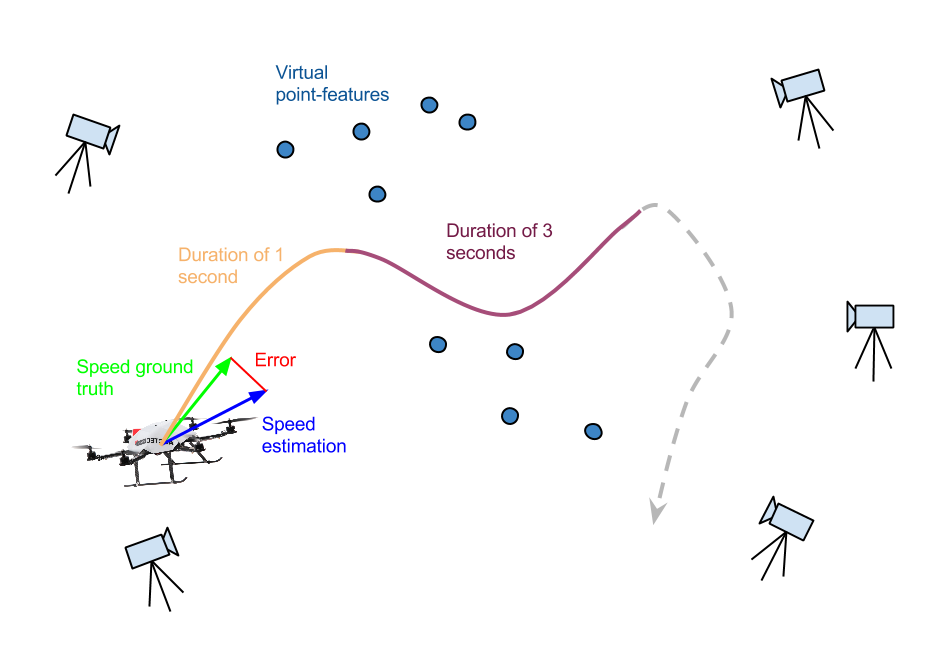
\includegraphics[width=\columnwidth]{images/setupTestDroneError.png}
\end{figure}

\subsection{Original performance}

\begin{figure}[h!]
  \centering
  \resizebox{0.7\columnwidth}{!}{% This file was created by matlab2tikz.
% Minimal pgfplots version: 1.3
%
%The latest updates can be retrieved from
%  http://www.mathworks.com/matlabcentral/fileexchange/22022-matlab2tikz
%where you can also make suggestions and rate matlab2tikz.
%
\definecolor{mycolor1}{rgb}{0,1,0}%
%
\begin{tikzpicture}

\begin{axis}[%
width=4.5in,
height=3.7in,
at={(1.751579in,1.09421in)},
scale only axis,
xmin=1.5,
xmax=4.5,
xlabel={Duration (s)},
ymin=0,
ymax=1,
ylabel={Error},
font=\tiny,
xtick={1.5,2,...,4,4.5},
ytick={0.1,0.2,...,1,1.1},
legend style={font=\tiny, legend cell align=left,align=left,draw=white!15!black},
label style={font=\tiny}
]
\addlegendimage{line legend,blue} % or mark=none?
\addlegendentry{Lambda}
\addlegendimage{line legend,red}
\addlegendentry{Speed}
\addlegendimage{line legend,color=mycolor1}
\addlegendentry{Gravity}
\addplot [color=blue,solid]
  table[row sep=crcr]{%
1.5	0.762801178696159\\
2	0.490854841841618\\
2.5	0.460758656914928\\
3	0.481813646472708\\
3.5	0.461642438720163\\
4	0.437968480311408\\
4.5	0.409852108955419\\
};

\addplot [color=red,solid,forget plot]
  table[row sep=crcr]{%
1.5	0.897783065827637\\
2	0.625026337752138\\
2.5	0.594488594286172\\
3	0.625761539018411\\
3.5	0.555488396593806\\
4	0.465559666180634\\
4.5	0.362061397104667\\
};
\addplot [color=mycolor1,solid,forget plot]
  table[row sep=crcr]{%
1.5	0.152942570020578\\
2	0.0888439460940633\\
2.5	0.0761934019897938\\
3	0.069897164835093\\
3.5	0.0546837789020217\\
4	0.0447432430773695\\
4.5	0.0350875815151695\\
};

\end{axis}
\end{tikzpicture}%
}
  %% \caption{Performance of the Original Closed-Form Solution}
\end{figure}

With around 45\% of error on the speed and the distance to the features after 4 seconds of integration, the Original Closed-Form Solution does not perform very well on terrain data.

\section{Impact of bias}
We studied the impact of biased inertial sensors on the performance of the original Closed-Form Solution.
by experimenting with real and synthetic data, we realized that the performance is:
\begin{itemize}
 \item Strongly affected by the gyroscope bias;
 \item Weakly affected by the accelerometer bias.
\end{itemize}

  \begin{figure}[h!]
    \caption{Speed estimation error}
    \centering
    \begin{subfigure}[b]{0.47\columnwidth}
      \resizebox{\columnwidth}{!}{% This file was created by matlab2tikz.
% Minimal pgfplots version: 1.3
%
%The latest updates can be retrieved from
%  http://www.mathworks.com/matlabcentral/fileexchange/22022-matlab2tikz
%where you can also make suggestions and rate matlab2tikz.
%
\begin{tikzpicture}

\begin{axis}[%
compat=newest,
width=3.7in,
height=3in,
at={(1.751579in,1.09421in)},
scale only axis,
xmin=1.5,
xmax=4.5,
xlabel={ Duration (s)},
ytick={0.1,0.2,...,1,1.1},
xtick={1.5,2,...,4,4.5},
font=\scriptsize,
ymin=0,
ymax=1,
ylabel={Error},
title style={font=\bfseries},
legend style={font=\small,legend cell align=left,align=left,draw=white!15!black}
]
\addplot [color=red,solid]
  table[row sep=crcr]{%
1.5	0.427463972747558\\
2	0.204392897471152\\
2.5	0.2086891919016\\
3	0.126226810629669\\
3.5	0.147352344834344\\
4	0.153986273651178\\
4.5	0.160248218913411\\
};
\addlegendentry{\textbar bias\textbar=0};

\addplot [color=green,solid]
  table[row sep=crcr]{%
1.5	0.427842146458304\\
2	0.20268073059906\\
2.5	0.208771544411042\\
3	0.129271147402759\\
3.5	0.148897086867292\\
4	0.154358837863052\\
4.5	0.16081022719229\\
};
\addlegendentry{\textbar bias\textbar =0.05};

\addplot [color=blue,solid]
  table[row sep=crcr]{%
1.5	0.429414835548993\\
2	0.20381870636079\\
2.5	0.219075218522201\\
3	0.128278996183278\\
3.5	0.144791652305567\\
4	0.157454176592355\\
4.5	0.144590793884469\\
};
\addlegendentry{\textbar bias\textbar=0.2};

\end{axis}
\end{tikzpicture}%
}
      \caption{Varying accelerometer bias}
    \end{subfigure}
    \begin{subfigure}[b]{0.47\columnwidth}
      \resizebox{\columnwidth}{!}{% This file was created by matlab2tikz.
% Minimal pgfplots version: 1.3
%
%The latest updates can be retrieved from
%  http://www.mathworks.com/matlabcentral/fileexchange/22022-matlab2tikz
%where you can also make suggestions and rate matlab2tikz.
%
\begin{tikzpicture}

\begin{axis}[%
compat=newest,
width=3.7in,
height=3in,
at={(1.751579in,1.09421in)},
scale only axis,
unbounded coords=jump,
xmin=1.5,
xmax=4.5,
font=\scriptsize,
xlabel={Duration (s)},
ytick={0.1,0.2,...,1,1.1},
xtick={1.5,2,...,4,4.5},
ymin=0,
ymax=1,
ylabel={Error },
title style={font=\bfseries},
legend style={font=\small,legend cell align=left,align=left,draw=white!15!black}
]
\addplot [color=red,solid]
  table[row sep=crcr]{%
1.5	0.69385799743164\\
1.79	0.351400106646042\\
2.08	0.208972359940106\\
2.37	0.189904693757416\\
2.66	0.155031673380865\\
2.95	0.156603969287685\\
3.24	0.152939916596076\\
3.53	0.150155750111395\\
3.82	0.15549617974511\\
4.11	0.152358693836919\\
4.4	0.148302651272463\\
4.69	0.142615204897316\\
};
\addlegendentry{\textbar bias\textbar =0};

\addplot [color=green,solid]
  table[row sep=crcr]{%
1.5	0.899343688689263\\
1.79	0.6670895311607\\
2.08	0.492994031916181\\
2.37	0.468605658830025\\
2.66	0.422315774521047\\
2.95	0.422348108072392\\
3.24	0.456442867280175\\
3.53	0.496882747914263\\
3.82	0.477797052531491\\
4.11	0.561139746296675\\
4.4	0.646949430497149\\
4.69	0.642082595006945\\
};
\addlegendentry{\textbar bias\textbar =0.05};

\addplot [color=blue,solid]
  table[row sep=crcr]{%
2.8434373353642	1.1\\
2.95	0.931895449882512\\
3.03721993366237	1.1\\
};
\addlegendentry{\textbar bias\textbar=0.2};

\node at (axis cs:3.5,0.3) {\color{blue}\textbar bias\textbar=0.2 off chart};

\end{axis}
\end{tikzpicture}%
}
      \caption{Varying gyroscope bias}
    \end{subfigure}
  \end{figure}


\section{Our method}

The goal is to factor out the gyroscope bias to improve the performance of the Closed-Form Solution.
Optimally, we would add the gyroscope bias as an unknown term in $X$.
Unfortunately we cannot express the gyroscope bias linearly with respect to the visual-inertial measurements.

We propose a different approach: a non-linear minimization of the residual with respect to the gyroscope bias.
In other words, we recover $X$ by minimizing the cost function:

\[
cost(B) = \argmin_X ||\Xi X - S||^2
\]
{\small \emph{With:\\
$B$ the gyroscope bias,\\
$\Xi$ and $S$ computed with respect to $B$}}

The gyroscope bias is a 3D vector $B=[B_x,B_y,B_z]$. We can plot this cost function with respect to two components of the gyroscope bias:
\begin{figure}[h!]
  \centering
  \resizebox{\columnwidth}{!}{% This file was created by matlab2tikz.
% Minimal pgfplots version: 1.3
%
%The latest updates can be retrieved from
%  http://www.mathworks.com/matlabcentral/fileexchange/22022-matlab2tikz
%where you can also make suggestions and rate matlab2tikz.
%
\begin{tikzpicture}

\begin{axis}[%
width=10.442105in,
height=8.107105in,
at={(0.921556in,1.181889in)},
scale only axis,
xmin=-2,
xmax=2,
tick align=outside,
xlabel={$B_x$ (rad/s)},
xmajorgrids,
ymin=-2,
ymax=2,
font=\tiny,
xtick={-2,-1.5,...,1.5,2},
ytick={-2,-1.5,...,1.5,2},
ylabel={$B_z$ (rad/s)},
zlabel={Residual},
ymajorgrids,
zmin=0,
zmax=8,
zmajorgrids,
view={-44.5}{20},
axis x line*=bottom,
axis y line*=left,
axis z line*=left
]

  \draw (axis cs:0,-1.1,0) node {\color{red} \large True bias} -> (axis cs:0.0800000000000001, 0.0800000000000001, 1.01510575861715);

\addplot3[%
surf,
faceted color=black,
shader=faceted,
colormap={mymap}{[1pt] rgb(0pt)=(0.2081,0.1663,0.5292); rgb(1pt)=(0.211624,0.189781,0.577676); rgb(2pt)=(0.212252,0.213771,0.626971); rgb(3pt)=(0.2081,0.2386,0.677086); rgb(4pt)=(0.195905,0.264457,0.7279); rgb(5pt)=(0.170729,0.291938,0.779248); rgb(6pt)=(0.125271,0.324243,0.830271); rgb(7pt)=(0.0591333,0.359833,0.868333); rgb(8pt)=(0.0116952,0.38751,0.881957); rgb(9pt)=(0.00595714,0.408614,0.882843); rgb(10pt)=(0.0165143,0.4266,0.878633); rgb(11pt)=(0.0328524,0.443043,0.871957); rgb(12pt)=(0.0498143,0.458571,0.864057); rgb(13pt)=(0.0629333,0.47369,0.855438); rgb(14pt)=(0.0722667,0.488667,0.8467); rgb(15pt)=(0.0779429,0.503986,0.838371); rgb(16pt)=(0.0793476,0.520024,0.831181); rgb(17pt)=(0.0749429,0.537543,0.826271); rgb(18pt)=(0.0640571,0.556986,0.823957); rgb(19pt)=(0.0487714,0.577224,0.822829); rgb(20pt)=(0.0343429,0.596581,0.819852); rgb(21pt)=(0.0265,0.6137,0.8135); rgb(22pt)=(0.0238905,0.628662,0.803762); rgb(23pt)=(0.0230905,0.641786,0.791267); rgb(24pt)=(0.0227714,0.653486,0.776757); rgb(25pt)=(0.0266619,0.664195,0.760719); rgb(26pt)=(0.0383714,0.674271,0.743552); rgb(27pt)=(0.0589714,0.683757,0.725386); rgb(28pt)=(0.0843,0.692833,0.706167); rgb(29pt)=(0.113295,0.7015,0.685857); rgb(30pt)=(0.145271,0.709757,0.664629); rgb(31pt)=(0.180133,0.717657,0.642433); rgb(32pt)=(0.217829,0.725043,0.619262); rgb(33pt)=(0.258643,0.731714,0.595429); rgb(34pt)=(0.302171,0.737605,0.571186); rgb(35pt)=(0.348167,0.742433,0.547267); rgb(36pt)=(0.395257,0.7459,0.524443); rgb(37pt)=(0.44201,0.748081,0.503314); rgb(38pt)=(0.487124,0.749062,0.483976); rgb(39pt)=(0.530029,0.749114,0.466114); rgb(40pt)=(0.570857,0.748519,0.44939); rgb(41pt)=(0.609852,0.747314,0.433686); rgb(42pt)=(0.6473,0.7456,0.4188); rgb(43pt)=(0.683419,0.743476,0.404433); rgb(44pt)=(0.71841,0.741133,0.390476); rgb(45pt)=(0.752486,0.7384,0.376814); rgb(46pt)=(0.785843,0.735567,0.363271); rgb(47pt)=(0.818505,0.732733,0.34979); rgb(48pt)=(0.850657,0.7299,0.336029); rgb(49pt)=(0.882433,0.727433,0.3217); rgb(50pt)=(0.913933,0.725786,0.306276); rgb(51pt)=(0.944957,0.726114,0.288643); rgb(52pt)=(0.973895,0.731395,0.266648); rgb(53pt)=(0.993771,0.745457,0.240348); rgb(54pt)=(0.999043,0.765314,0.216414); rgb(55pt)=(0.995533,0.786057,0.196652); rgb(56pt)=(0.988,0.8066,0.179367); rgb(57pt)=(0.978857,0.827143,0.163314); rgb(58pt)=(0.9697,0.848138,0.147452); rgb(59pt)=(0.962586,0.870514,0.1309); rgb(60pt)=(0.958871,0.8949,0.113243); rgb(61pt)=(0.959824,0.921833,0.0948381); rgb(62pt)=(0.9661,0.951443,0.0755333); rgb(63pt)=(0.9763,0.9831,0.0538)},
mesh/rows=51]
table[row sep=crcr,header=false] {%
%
-2	-2	3.96953559596561\\
-2	-1.92	4.10768647002591\\
-2	-1.84	4.24569847297076\\
-2	-1.76	4.3840218213466\\
-2	-1.68	4.52305616147229\\
-2	-1.6	4.66307817919315\\
-2	-1.52	4.80418369276614\\
-2	-1.44	4.94625064166626\\
-2	-1.36	5.08892766050472\\
-2	-1.28	5.23165000647402\\
-2	-1.2	5.37368084411246\\
-2	-1.12	5.51417201162251\\
-2	-1.04	5.65223532899549\\
-2	-0.96	5.78701409946557\\
-2	-0.88	5.91774508904903\\
-2	-0.8	6.04380361330781\\
-2	-0.72	6.16472743291698\\
-2	-0.64	6.28021782446951\\
-2	-0.56	6.39011787978065\\
-2	-0.48	6.49436921231523\\
-2	-0.4	6.59294989381992\\
-2	-0.32	6.68579940086098\\
-2	-0.24	6.77274030366729\\
-2	-0.16	6.85340998046518\\
-2	-0.0800000000000001	6.92721707426617\\
-2	0	6.99333544574209\\
-2	0.0800000000000001	7.05074252721512\\
-2	0.16	7.09829983478544\\
-2	0.24	7.13486298666621\\
-2	0.32	7.15940026194346\\
-2	0.4	7.17109590087901\\
-2	0.48	7.16941848756345\\
-2	0.56	7.15414442647747\\
-2	0.64	7.12533813500834\\
-2	0.72	7.08330030278077\\
-2	0.8	7.02850093029741\\
-2	0.88	6.96151416647848\\
-2	0.96	6.88296800946441\\
-2	1.04	6.79351545772275\\
-2	1.12	6.69382684182674\\
-2	1.2	6.58459778282305\\
-2	1.28	6.46656469268609\\
-2	1.36	6.34052002784537\\
-2	1.44	6.20732170347499\\
-2	1.52	6.06789381913412\\
-2	1.6	5.9232180635586\\
-2	1.68	5.77431649081623\\
-2	1.76	5.62222704624045\\
-2	1.84	5.46797373702601\\
-2	1.92	5.31253397981478\\
-2	2	5.15680635884562\\
-1.92	-2	4.12256554777728\\
-1.92	-1.92	4.26668432204039\\
-1.92	-1.84	4.41087178326284\\
-1.92	-1.76	4.55542689958074\\
-1.92	-1.68	4.70052423361521\\
-1.92	-1.6	4.84615330214983\\
-1.92	-1.52	4.99207973536112\\
-1.92	-1.44	5.13783397629943\\
-1.92	-1.36	5.2827306352235\\
-1.92	-1.28	5.42591774877334\\
-1.92	-1.2	5.56645052138299\\
-1.92	-1.12	5.7033796130576\\
-1.92	-1.04	5.83584103863677\\
-1.92	-0.96	5.96313446784647\\
-1.92	-0.88	6.08477949096741\\
-1.92	-0.8	6.20054423823241\\
-1.92	-0.72	6.31044557436716\\
-1.92	-0.64	6.41472294711033\\
-1.92	-0.56	6.5137882238851\\
-1.92	-0.48	6.60815282316808\\
-1.92	-0.4	6.69833359986875\\
-1.92	-0.32	6.78474207655356\\
-1.92	-0.24	6.86756747660566\\
-1.92	-0.16	6.94667051861043\\
-1.92	-0.0800000000000001	7.02150941909083\\
-1.92	0	7.0911196745187\\
-1.92	0.0800000000000001	7.15416304991952\\
-1.92	0.16	7.20904800422466\\
-1.92	0.24	7.2541055973428\\
-1.92	0.32	7.28778763995639\\
-1.92	0.4	7.30884505616819\\
-1.92	0.48	7.31644880345962\\
-1.92	0.56	7.31023172356702\\
-1.92	0.64	7.29025081294116\\
-1.92	0.72	7.25688814385105\\
-1.92	0.8	7.21072011503312\\
-1.92	0.88	7.15238731759473\\
-1.92	0.96	7.08249211531543\\
-1.92	1.04	7.00154068237248\\
-1.92	1.12	6.90993401657131\\
-1.92	1.2	6.80800144816006\\
-1.92	1.28	6.6960625463911\\
-1.92	1.36	6.57449994876512\\
-1.92	1.44	6.4438261781428\\
-1.92	1.52	6.30473091971276\\
-1.92	1.6	6.15810030142864\\
-1.92	1.68	6.00500547663265\\
-1.92	1.76	5.84666343023339\\
-1.92	1.84	5.68437752083278\\
-1.92	1.92	5.51946793219248\\
-1.92	2	5.35320252672805\\
-1.84	-2	4.26817660315442\\
-1.84	-1.92	4.41756364181435\\
-1.84	-1.84	4.56692433772459\\
-1.84	-1.76	4.71628611412794\\
-1.84	-1.68	4.86548461712527\\
-1.84	-1.6	5.01412551775112\\
-1.84	-1.52	5.16157591177941\\
-1.84	-1.44	5.30698926125651\\
-1.84	-1.36	5.4493641076256\\
-1.84	-1.28	5.5876316473392\\
-1.84	-1.2	5.72076142350429\\
-1.84	-1.12	5.84786958026397\\
-1.84	-1.04	5.96831253042371\\
-1.84	-0.96	6.08175189141002\\
-1.84	-0.88	6.18818356533774\\
-1.84	-0.8	6.28793212190221\\
-1.84	-0.72	6.38161744791494\\
-1.84	-0.64	6.47010129010687\\
-1.84	-0.56	6.55441705352494\\
-1.84	-0.48	6.63568041865717\\
-1.84	-0.4	6.71497573179798\\
-1.84	-0.32	6.79321669562466\\
-1.84	-0.24	6.87098905305687\\
-1.84	-0.16	6.94839457713728\\
-1.84	-0.0800000000000001	7.02492631688921\\
-1.84	0	7.09941135021931\\
-1.84	0.0800000000000001	7.1700546492594\\
-1.84	0.16	7.2346010696438\\
-1.84	0.24	7.29060169056717\\
-1.84	0.32	7.33573531066088\\
-1.84	0.4	7.36811262527784\\
-1.84	0.48	7.38649242352188\\
-1.84	0.56	7.39036540846271\\
-1.84	0.64	7.37989910161782\\
-1.84	0.72	7.35577158108122\\
-1.84	0.8	7.31894303899675\\
-1.84	0.88	7.27041980958118\\
-1.84	0.96	7.21105787839203\\
-1.84	1.04	7.14143685320625\\
-1.84	1.12	7.06181672429096\\
-1.84	1.2	6.97217322641791\\
-1.84	1.28	6.87229572586919\\
-1.84	1.36	6.76192453410124\\
-1.84	1.44	6.64090143060214\\
-1.84	1.52	6.50930702267799\\
-1.84	1.6	6.36756123818174\\
-1.84	1.68	6.21646936578914\\
-1.84	1.76	6.05720606396812\\
-1.84	1.84	5.89124243832386\\
-1.84	1.92	5.72023316228771\\
-1.84	2	5.54588746760841\\
-1.76	-2	4.40328552747556\\
-1.76	-1.92	4.55670966374549\\
-1.76	-1.84	4.70956836166359\\
-1.76	-1.76	4.86150661116584\\
-1.76	-1.68	5.01193114339525\\
-1.76	-1.6	5.16000799368019\\
-1.76	-1.52	5.30469706382988\\
-1.76	-1.44	5.44482386110451\\
-1.76	-1.36	5.57918305009132\\
-1.76	-1.28	5.70666162048795\\
-1.76	-1.2	5.82636319868087\\
-1.76	-1.12	5.93771230323948\\
-1.76	-1.04	6.04052067465287\\
-1.76	-0.96	6.13500726588581\\
-1.76	-0.88	6.22177589121777\\
-1.76	-0.8	6.30176465415031\\
-1.76	-0.72	6.37618432216034\\
-1.76	-0.64	6.44645696895032\\
-1.76	-0.56	6.51415400079994\\
-1.76	-0.48	6.5809204388966\\
-1.76	-0.4	6.64836707175863\\
-1.76	-0.32	6.71791724518849\\
-1.76	-0.24	6.79060868127472\\
-1.76	-0.16	6.86686864946821\\
-1.76	-0.0800000000000001	6.94630065196898\\
-1.76	0	7.02754018327651\\
-1.76	0.0800000000000001	7.10824746702435\\
-1.76	0.16	7.18529071848165\\
-1.76	0.24	7.25512419637796\\
-1.76	0.32	7.31429391901961\\
-1.76	0.4	7.3599471292927\\
-1.76	0.48	7.39021384584179\\
-1.76	0.56	7.40437336681156\\
-1.76	0.64	7.40278797126489\\
-1.76	0.72	7.38664786417496\\
-1.76	0.8	7.35760776173661\\
-1.76	0.88	7.31740364183628\\
-1.76	0.96	7.2675236932963\\
-1.76	1.04	7.20898020494889\\
-1.76	1.12	7.14220010385522\\
-1.76	1.2	7.06702945291546\\
-1.76	1.28	6.98283432714661\\
-1.76	1.36	6.8886749061129\\
-1.76	1.44	6.78352690162109\\
-1.76	1.52	6.66652100673566\\
-1.76	1.6	6.53716629256946\\
-1.76	1.68	6.39552039526287\\
-1.76	1.76	6.24227325198951\\
-1.76	1.84	6.07872609892112\\
-1.76	1.92	5.90667171126118\\
-1.76	2	5.72820663959609\\
-1.68	-2	4.52442817444724\\
-1.68	-1.92	4.6800196488908\\
-1.68	-1.84	4.83395797726146\\
-1.68	-1.76	4.98542947430613\\
-1.68	-1.68	5.13337717696746\\
-1.68	-1.6	5.27654994518269\\
-1.68	-1.52	5.41359285621812\\
-1.68	-1.44	5.54317100012462\\
-1.68	-1.36	5.66411102282432\\
-1.68	-1.28	5.77553786095503\\
-1.68	-1.2	5.8769814409298\\
-1.68	-1.12	5.96843276499073\\
-1.68	-1.04	6.05034111884961\\
-1.68	-0.96	6.12356048389156\\
-1.68	-0.88	6.18926737189971\\
-1.68	-0.8	6.24887833552567\\
-1.68	-0.72	6.303990328886\\
-1.68	-0.64	6.35635180234238\\
-1.68	-0.56	6.40785192524329\\
-1.68	-0.48	6.46049798270151\\
-1.68	-0.4	6.51634492297579\\
-1.68	-0.32	6.57734855745127\\
-1.68	-0.24	6.64513029621805\\
-1.68	-0.16	6.72066221251066\\
-1.68	-0.0800000000000001	6.80391030942226\\
-1.68	0	6.89351649114508\\
-1.68	0.0800000000000001	6.98664419647848\\
-1.68	0.16	7.07912021833977\\
-1.68	0.24	7.16593429510817\\
-1.68	0.32	7.24201644126465\\
-1.68	0.4	7.30307877418483\\
-1.68	0.48	7.34627449764164\\
-1.68	0.56	7.37050799261757\\
-1.68	0.64	7.37636255036981\\
-1.68	0.72	7.36572298957398\\
-1.68	0.8	7.34122782555508\\
-1.68	0.88	7.30569250291519\\
-1.68	0.96	7.26161540018844\\
-1.68	1.04	7.21082966139778\\
-1.68	1.12	7.15431621098008\\
-1.68	1.2	7.09216157331658\\
-1.68	1.28	7.02363249018917\\
-1.68	1.36	6.94734204521142\\
-1.68	1.44	6.86148901478261\\
-1.68	1.52	6.76415436060813\\
-1.68	1.6	6.65363112862622\\
-1.68	1.68	6.52874765896951\\
-1.68	1.76	6.38912743892591\\
-1.68	1.84	6.23532585230776\\
-1.68	1.92	6.06880540637501\\
-1.68	2	5.8917542370859\\
-1.6	-2	4.62778433556879\\
-1.6	-1.92	4.78301319347452\\
-1.6	-1.84	4.93492304277036\\
-1.6	-1.76	5.0822352271011\\
-1.6	-1.68	5.22349124598085\\
-1.6	-1.6	5.35716776034462\\
-1.6	-1.52	5.48182661935434\\
-1.6	-1.44	5.59627747185312\\
-1.6	-1.36	5.69972370273108\\
-1.6	-1.28	5.79186192975515\\
-1.6	-1.2	5.87291363455427\\
-1.6	-1.12	5.94358395450792\\
-1.6	-1.04	6.00496239199529\\
-1.6	-0.96	6.05839621134074\\
-1.6	-0.88	6.10537405301387\\
-1.6	-0.8	6.14745292132042\\
-1.6	-0.72	6.1862472936714\\
-1.6	-0.64	6.22347725320662\\
-1.6	-0.56	6.26104803911255\\
-1.6	-0.48	6.30111459754974\\
-1.6	-0.4	6.3460798676179\\
-1.6	-0.32	6.39848413251494\\
-1.6	-0.24	6.46075466632553\\
-1.6	-0.16	6.53479631643089\\
-1.6	-0.0800000000000001	6.62143312995678\\
-1.6	0	6.71978784984478\\
-1.6	0.0800000000000001	6.82680587560688\\
-1.6	0.16	6.93721320640349\\
-1.6	0.24	7.04411840830546\\
-1.6	0.32	7.14019268379049\\
-1.6	0.4	7.21905448876112\\
-1.6	0.48	7.27638437867899\\
-1.6	0.56	7.31045965338174\\
-1.6	0.64	7.32206531858272\\
-1.6	0.72	7.31393311867062\\
-1.6	0.8	7.28993686235302\\
-1.6	0.88	7.25426395905756\\
-1.6	0.96	7.21072523432045\\
-1.6	1.04	7.16228319105905\\
-1.6	1.12	7.11080196411066\\
-1.6	1.2	7.05697503403306\\
-1.6	1.28	7.00037590577109\\
-1.6	1.36	6.93959190493738\\
-1.6	1.44	6.87242545738576\\
-1.6	1.52	6.79616629102195\\
-1.6	1.6	6.70794166830724\\
-1.6	1.68	6.60513437344105\\
-1.6	1.76	6.48582207886236\\
-1.6	1.84	6.34915225324422\\
-1.6	1.92	6.19555092610987\\
-1.6	2	6.02669441494223\\
-1.52	-2	4.70933426963172\\
-1.52	-1.92	4.86111721999925\\
-1.52	-1.84	5.00742868293308\\
-1.52	-1.76	5.14663129961776\\
-1.52	-1.68	5.2770661124964\\
-1.52	-1.6	5.39723432113434\\
-1.52	-1.52	5.50598518566188\\
-1.52	-1.44	5.60267008085075\\
-1.52	-1.36	5.68722645874004\\
-1.52	-1.28	5.76017108870496\\
-1.52	-1.2	5.82250525198233\\
-1.52	-1.12	5.87555771397464\\
-1.52	-1.04	5.92080636128271\\
-1.52	-0.96	5.95972246669853\\
-1.52	-0.88	5.9936742095144\\
-1.52	-0.8	6.02391267885352\\
-1.52	-0.72	6.05164671704268\\
-1.52	-0.64	6.07819224530468\\
-1.52	-0.56	6.10515864429766\\
-1.52	-0.48	6.13461778771808\\
-1.52	-0.4	6.16919962742021\\
-1.52	-0.32	6.21206566411352\\
-1.52	-0.24	6.26670637249846\\
-1.52	-0.16	6.33648452027554\\
-1.52	-0.0800000000000001	6.42384710839879\\
-1.52	0	6.52923856098694\\
-1.52	0.0800000000000001	6.65001001014032\\
-1.52	0.16	6.77990310067574\\
-1.52	0.24	6.9096676259882\\
-1.52	0.32	7.02884931480038\\
-1.52	0.4	7.12807822273418\\
-1.52	0.48	7.20092269373549\\
-1.52	0.56	7.24473595806138\\
-1.52	0.64	7.26048829975158\\
-1.52	0.72	7.25191169902747\\
-1.52	0.8	7.22434044449202\\
-1.52	0.88	7.18356447069955\\
-1.52	0.96	7.13491127083845\\
-1.52	1.04	7.08265296273149\\
-1.52	1.12	7.02972217672927\\
-1.52	1.2	6.97765122555585\\
-1.52	1.28	6.92663656953075\\
-1.52	1.36	6.87565832256273\\
-1.52	1.44	6.82262736353079\\
-1.52	1.52	6.76457230581171\\
-1.52	1.6	6.69790411332315\\
-1.52	1.68	6.61879799770635\\
-1.52	1.76	6.52370122428568\\
-1.52	1.84	6.40991160647632\\
-1.52	1.92	6.27609808879832\\
-1.52	2	6.12259992432149\\
-1.44	-2	4.76516754626026\\
-1.44	-1.92	4.91014143160211\\
-1.44	-1.84	5.04726045704531\\
-1.44	-1.76	5.17478187628494\\
-1.44	-1.68	5.29120071377539\\
-1.44	-1.6	5.39546671574785\\
-1.44	-1.52	5.4871480755165\\
-1.44	-1.44	5.56649547717501\\
-1.44	-1.36	5.63438647887661\\
-1.44	-1.28	5.69216451968405\\
-1.44	-1.2	5.74141489744198\\
-1.44	-1.12	5.78373214574672\\
-1.44	-1.04	5.82052821588824\\
-1.44	-0.96	5.85291541780824\\
-1.44	-0.88	5.88168159782855\\
-1.44	-0.8	5.90736310200905\\
-1.44	-0.72	5.93041144025602\\
-1.44	-0.64	5.95143534095639\\
-1.44	-0.56	5.9714803967029\\
-1.44	-0.48	5.99229649977898\\
-1.44	-0.4	6.0165505641151\\
-1.44	-0.32	6.04795086807774\\
-1.44	-0.24	6.0912139061929\\
-1.44	-0.16	6.1517042747166\\
-1.44	-0.0800000000000001	6.23448280278144\\
-1.44	0	6.34259321221886\\
-1.44	0.0800000000000001	6.47490205657937\\
-1.44	0.16	6.62455348089451\\
-1.44	0.24	6.77936912550455\\
-1.44	0.32	6.92457530198942\\
-1.44	0.4	7.04662965620654\\
-1.44	0.48	7.13625656921428\\
-1.44	0.56	7.18964958522293\\
-1.44	0.64	7.20803571878708\\
-1.44	0.72	7.19633523715703\\
-1.44	0.8	7.16154204826462\\
-1.44	0.88	7.11121343776957\\
-1.44	0.96	7.0523057213835\\
-1.44	1.04	6.99046251123338\\
-1.44	1.12	6.92972214874134\\
-1.44	1.2	6.87251282455348\\
-1.44	1.28	6.81978394200449\\
-1.44	1.36	6.77116125001577\\
-1.44	1.44	6.72507299723181\\
-1.44	1.52	6.67885055672692\\
-1.44	1.6	6.62885173148658\\
-1.44	1.68	6.57068386086243\\
-1.44	1.76	6.4996047329644\\
-1.44	1.84	6.41113289161592\\
-1.44	1.92	6.30179785588019\\
-1.44	2	6.16983959189987\\
-1.36	-2	4.79193510933177\\
-1.36	-1.92	4.92690912333141\\
-1.36	-1.84	5.05184763044736\\
-1.36	-1.76	5.16529954112991\\
-1.36	-1.68	5.26637243182022\\
-1.36	-1.6	5.35490885581798\\
-1.36	-1.52	5.43153120210487\\
-1.36	-1.44	5.49753278268912\\
-1.36	-1.36	5.55464250395734\\
-1.36	-1.28	5.60472675773468\\
-1.36	-1.2	5.64950104203768\\
-1.36	-1.12	5.69030791912322\\
-1.36	-1.04	5.72799063378592\\
-1.36	-0.96	5.76286772091805\\
-1.36	-0.88	5.79480213032436\\
-1.36	-0.8	5.82335787227862\\
-1.36	-0.72	5.84803740614665\\
-1.36	-0.64	5.86858253327152\\
-1.36	-0.56	5.88530441862654\\
-1.36	-0.48	5.89940882992179\\
-1.36	-0.4	5.91331496859406\\
-1.36	-0.32	5.93099124221408\\
-1.36	-0.24	5.95826407853514\\
-1.36	-0.16	6.00283539251812\\
-1.36	-0.0800000000000001	6.07343104981368\\
-1.36	0	6.17741396305353\\
-1.36	0.0800000000000001	6.31691864544529\\
-1.36	0.16	6.48526724658617\\
-1.36	0.24	6.66662212185912\\
-1.36	0.32	6.84021630903693\\
-1.36	0.4	6.98684422533705\\
-1.36	0.48	7.09372665807658\\
-1.36	0.56	7.15593445652366\\
-1.36	0.64	7.17523585975184\\
-1.36	0.72	7.15797349196666\\
-1.36	0.8	7.11292291191939\\
-1.36	0.88	7.04945885646163\\
-1.36	0.96	6.97617473503991\\
-1.36	1.04	6.90005567574021\\
-1.36	1.12	6.82618163628421\\
-1.36	1.2	6.75780143768638\\
-1.36	1.28	6.69657315188477\\
-1.36	1.36	6.64280925703333\\
-1.36	1.44	6.59564042700969\\
-1.36	1.52	6.55308052729573\\
-1.36	1.6	6.5120296092844\\
-1.36	1.68	6.46829735323853\\
-1.36	1.76	6.41676523165552\\
-1.36	1.84	6.3518100600053\\
-1.36	1.92	6.26804671907927\\
-1.36	2	6.16129453428772\\
-1.28	-2	4.78738447915804\\
-1.28	-1.92	4.90992667692113\\
-1.28	-1.84	5.02101776365417\\
-1.28	-1.76	5.11996922553663\\
-1.28	-1.68	5.2069367448633\\
-1.28	-1.6	5.28295098511002\\
-1.28	-1.52	5.34975807868581\\
-1.28	-1.44	5.40950786396655\\
-1.28	-1.36	5.46437703222833\\
-1.28	-1.28	5.51622173766807\\
-1.28	-1.2	5.56632642577357\\
-1.28	-1.12	5.61527544193304\\
-1.28	-1.04	5.66294138506957\\
-1.28	-0.96	5.70856889677018\\
-1.28	-0.88	5.75093451594869\\
-1.28	-0.8	5.78857265020021\\
-1.28	-0.72	5.82005832733899\\
-1.28	-0.64	5.84432099147262\\
-1.28	-0.56	5.86095025040181\\
-1.28	-0.48	5.87048529296831\\
-1.28	-0.4	5.87476338615002\\
-1.28	-0.32	5.87747009978921\\
-1.28	-0.24	5.88495985149855\\
-1.28	-0.16	5.90706781062021\\
-1.28	-0.0800000000000001	5.95695002994464\\
-1.28	0	6.04831889050851\\
-1.28	0.0800000000000001	6.1891184643068\\
-1.28	0.16	6.37413271259019\\
-1.28	0.24	6.58279378673613\\
-1.28	0.32	6.78596508998077\\
-1.28	0.4	6.95709786309585\\
-1.28	0.48	7.07971606222367\\
-1.28	0.56	7.14842754229023\\
-1.28	0.64	7.16617894463176\\
-1.28	0.72	7.14097664956798\\
-1.28	0.8	7.08330374946679\\
-1.28	0.88	7.00417392190881\\
-1.28	0.96	6.91366180037765\\
-1.28	1.04	6.81997471894516\\
-1.28	1.12	6.7291185715046\\
-1.28	1.2	6.64502972959083\\
-1.28	1.28	6.56993389413044\\
-1.28	1.36	6.50471677174642\\
-1.28	1.44	6.44917973242329\\
-1.28	1.52	6.40213667331843\\
-1.28	1.6	6.36136708048894\\
-1.28	1.68	6.32348746912913\\
-1.28	1.76	6.283854626605\\
-1.28	1.84	6.23666538175282\\
-1.28	1.92	6.17542968364017\\
-1.28	2	6.09390014556686\\
-1.2	-2	4.7508538605985\\
-1.2	-1.92	4.85989099159592\\
-1.2	-1.84	4.95739049093819\\
-1.2	-1.76	5.0438351102545\\
-1.2	-1.68	5.12067284971446\\
-1.2	-1.6	5.19011587775703\\
-1.2	-1.52	5.25475705053877\\
-1.2	-1.44	5.31711398353346\\
-1.2	-1.36	5.37921968284093\\
-1.2	-1.28	5.4423378554967\\
-1.2	-1.2	5.50682767623097\\
-1.2	-1.12	5.57214536100751\\
-1.2	-1.04	5.63695426025783\\
-1.2	-0.96	5.69931599184915\\
-1.2	-0.88	5.75694386187062\\
-1.2	-0.8	5.80750262012935\\
-1.2	-0.72	5.84892158965712\\
-1.2	-0.64	5.87966041524665\\
-1.2	-0.56	5.89887445435089\\
-1.2	-0.48	5.90651679495754\\
-1.2	-0.4	5.9035664121382\\
-1.2	-0.32	5.89269590059884\\
-1.2	-0.24	5.87966878525935\\
-1.2	-0.16	5.87538539571144\\
-1.2	-0.0800000000000001	5.89739043000442\\
-1.2	0	5.96773716994066\\
-1.2	0.0800000000000001	6.1036096953683\\
-1.2	0.16	6.30313509297875\\
-1.2	0.24	6.53918783939804\\
-1.2	0.32	6.77087605478673\\
-1.2	0.4	6.96288525336062\\
-1.2	0.48	7.096063796809\\
-1.2	0.56	7.16625768815506\\
-1.2	0.64	7.17861739253798\\
-1.2	0.72	7.14293293736946\\
-1.2	0.8	7.07096983849761\\
-1.2	0.88	6.97483682834087\\
-1.2	0.96	6.8656752670254\\
-1.2	1.04	6.75267022016841\\
-1.2	1.12	6.64260646568057\\
-1.2	1.2	6.539977870396\\
-1.2	1.28	6.44742551383962\\
-1.2	1.36	6.366236795397\\
-1.2	1.44	6.29672529203921\\
-1.2	1.52	6.23841444470785\\
-1.2	1.6	6.19001704321929\\
-1.2	1.68	6.14924526068878\\
-1.2	1.76	6.11253104250449\\
-1.2	1.84	6.07480408092864\\
-1.2	1.92	6.02955153455922\\
-1.2	2	5.96940154450967\\
-1.12	-2	4.68355469138441\\
-1.12	-1.92	4.77980591923563\\
-1.12	-1.84	4.86615361279879\\
-1.12	-1.76	4.94444234832442\\
-1.12	-1.68	5.01733540185891\\
-1.12	-1.6	5.08786886930593\\
-1.12	-1.52	5.1589205052565\\
-1.12	-1.44	5.23274086285163\\
-1.12	-1.36	5.31063617918911\\
-1.12	-1.28	5.39281845091139\\
-1.12	-1.2	5.47839987668788\\
-1.12	-1.12	5.56550784150925\\
-1.12	-1.04	5.6515063692698\\
-1.12	-0.96	5.73331203182517\\
-1.12	-0.88	5.8077803056899\\
-1.12	-0.8	5.87210673645371\\
-1.12	-0.72	5.92414249468463\\
-1.12	-0.64	5.96250881786739\\
-1.12	-0.56	5.98646875363173\\
-1.12	-0.48	5.99568157853614\\
-1.12	-0.4	5.99015320471935\\
-1.12	-0.32	5.97084365294417\\
-1.12	-0.24	5.94149025503613\\
-1.12	-0.16	5.91207362261711\\
-1.12	-0.0800000000000001	5.9031369305011\\
-1.12	0	5.94636881328439\\
-1.12	0.0800000000000001	6.07245025260633\\
-1.12	0.16	6.28532794462469\\
-1.12	0.24	6.54794850443774\\
-1.12	0.32	6.80306635145794\\
-1.12	0.4	7.00657905596602\\
-1.12	0.48	7.13994173512807\\
-1.12	0.56	7.20311778778113\\
-1.12	0.64	7.20456183856677\\
-1.12	0.72	7.15559076690285\\
-1.12	0.8	7.06837649395873\\
-1.12	0.88	6.95517123594181\\
-1.12	0.96	6.82746056401677\\
-1.12	1.04	6.69499093351363\\
-1.12	1.12	6.56513115257047\\
-1.12	1.2	6.44282812766607\\
-1.12	1.28	6.33103077956345\\
-1.12	1.36	6.2312807248863\\
-1.12	1.44	6.14422048397617\\
-1.12	1.52	6.06989430765868\\
-1.12	1.6	6.00780877049394\\
-1.12	1.68	5.95676591142165\\
-1.12	1.76	5.91451204129216\\
-1.12	1.84	5.87729883831318\\
-1.12	1.92	5.83955090011633\\
-1.12	2	5.79394451861741\\
-1.04	-2	4.58848615271725\\
-1.04	-1.92	4.67455749102779\\
-1.04	-1.84	4.75415166006668\\
-1.04	-1.76	4.83034578412379\\
-1.04	-1.68	4.90659913725516\\
-1.04	-1.6	4.98614559589235\\
-1.04	-1.52	5.07146606722726\\
-1.04	-1.44	5.16395550016462\\
-1.04	-1.36	5.26377945007865\\
-1.04	-1.28	5.36985559572936\\
-1.04	-1.2	5.47992506106248\\
-1.04	-1.12	5.59073774001151\\
-1.04	-1.04	5.69839580316641\\
-1.04	-0.96	5.79885936392639\\
-1.04	-0.88	5.88853696170887\\
-1.04	-0.8	5.96479507673942\\
-1.04	-0.72	6.02618060706977\\
-1.04	-0.64	6.07222454072039\\
-1.04	-0.56	6.10288546400103\\
-1.04	-0.48	6.11789425420414\\
-1.04	-0.4	6.11637992339035\\
-1.04	-0.32	6.09724977226803\\
-1.04	-0.24	6.06104993490481\\
-1.04	-0.16	6.01445708460226\\
-1.04	-0.0800000000000001	5.97806642678256\\
-1.04	0	5.99278780252876\\
-1.04	0.0800000000000001	6.10730794779412\\
-1.04	0.16	6.33410629631957\\
-1.04	0.24	6.62011768380987\\
-1.04	0.32	6.88669600583211\\
-1.04	0.4	7.08471657226935\\
-1.04	0.48	7.20250284875729\\
-1.04	0.56	7.2473403264342\\
-1.04	0.64	7.23129634251376\\
-1.04	0.72	7.16626331071925\\
-1.04	0.8	7.0635611198274\\
-1.04	0.88	6.93439771051691\\
-1.04	0.96	6.78967602873492\\
-1.04	1.04	6.63912733406958\\
-1.04	1.12	6.49043442807225\\
-1.04	1.2	6.34890102078966\\
-1.04	1.28	6.21773223396025\\
-1.04	1.36	6.09864160177807\\
-1.04	1.44	5.99246237741676\\
-1.04	1.52	5.8995699850351\\
-1.04	1.6	5.82004908958863\\
-1.04	1.68	5.753603091807\\
-1.04	1.76	5.69922561947537\\
-1.04	1.84	5.65467964791347\\
-1.04	1.92	5.61590657299557\\
-1.04	2	5.57663181112982\\
-0.96	-2	4.46992092469625\\
-0.96	-1.92	4.54997522385874\\
-0.96	-1.84	4.62847809473426\\
-0.96	-1.76	4.70929764179712\\
-0.96	-1.68	4.7960266585906\\
-0.96	-1.6	4.89136411672159\\
-0.96	-1.52	4.9967621605839\\
-0.96	-1.44	5.11234640984927\\
-0.96	-1.36	5.23696608447713\\
-0.96	-1.28	5.36824074601927\\
-0.96	-1.2	5.50261597438129\\
-0.96	-1.12	5.63557488787122\\
-0.96	-1.04	5.7621484607368\\
-0.96	-0.96	5.87771002530049\\
-0.96	-0.88	5.97882391011489\\
-0.96	-0.8	6.0637878643383\\
-0.96	-0.72	6.13257986484576\\
-0.96	-0.64	6.18619018524292\\
-0.96	-0.56	6.22561620811828\\
-0.96	-0.48	6.2509135856649\\
-0.96	-0.4	6.26062667605742\\
-0.96	-0.32	6.25189614844014\\
-0.96	-0.24	6.22190069716201\\
-0.96	-0.16	6.17235942559362\\
-0.96	-0.0800000000000001	6.12007775911555\\
-0.96	0	6.11199105767275\\
-0.96	0.0800000000000001	6.2178215002422\\
-0.96	0.16	6.46000379711696\\
-0.96	0.24	6.75958612173297\\
-0.96	0.32	7.01494462211957\\
-0.96	0.4	7.18297867162666\\
-0.96	0.48	7.26673823038579\\
-0.96	0.56	7.28193765100006\\
-0.96	0.64	7.24266431005984\\
-0.96	0.72	7.15965533732045\\
-0.96	0.8	7.04204962163863\\
-0.96	0.88	6.89896228999232\\
-0.96	0.96	6.73986135235597\\
-0.96	1.04	6.57385380378386\\
-0.96	1.12	6.40860465160061\\
-0.96	1.2	6.24965572275522\\
-0.96	1.28	6.10044631045463\\
-0.96	1.36	5.96284105995568\\
-0.96	1.44	5.83779380260085\\
-0.96	1.52	5.72587268911135\\
-0.96	1.6	5.62753263518657\\
-0.96	1.68	5.54312027331214\\
-0.96	1.76	5.47262402250391\\
-0.96	1.84	5.4151826134034\\
-0.96	1.92	5.36839981444405\\
-0.96	2	5.32763520262829\\
-0.88	-2	4.33255252475105\\
-0.88	-1.92	4.41160365111778\\
-0.88	-1.84	4.49495387759301\\
-0.88	-1.76	4.58662727845616\\
-0.88	-1.68	4.68961558973461\\
-0.88	-1.6	4.80540150176895\\
-0.88	-1.52	4.93391655406888\\
-0.88	-1.44	5.07379289762823\\
-0.88	-1.36	5.22260470452363\\
-0.88	-1.28	5.37690529536106\\
-0.88	-1.2	5.53216372947175\\
-0.88	-1.12	5.6829408256254\\
-0.88	-1.04	5.82359437447953\\
-0.88	-0.96	5.94943498060895\\
-0.88	-0.88	6.05782401773185\\
-0.88	-0.8	6.14859588236381\\
-0.88	-0.72	6.22353636215807\\
-0.88	-0.64	6.28518469683672\\
-0.88	-0.56	6.33551916676949\\
-0.88	-0.48	6.37496978775241\\
-0.88	-0.4	6.40190051484762\\
-0.88	-0.32	6.41257206532109\\
-0.88	-0.24	6.40195292613502\\
-0.88	-0.16	6.36713461338936\\
-0.88	-0.0800000000000001	6.31830809639548\\
-0.88	0	6.30235810365394\\
-0.88	0.0800000000000001	6.40800390027246\\
-0.88	0.16	6.66340690004513\\
-0.88	0.24	6.95172722398527\\
-0.88	0.32	7.16053357883105\\
-0.88	0.4	7.27176441942384\\
-0.88	0.48	7.30668971211091\\
-0.88	0.56	7.28548262897892\\
-0.88	0.64	7.22058749801683\\
-0.88	0.72	7.11963487267072\\
-0.88	0.8	6.98869961629313\\
-0.88	0.88	6.83430104254152\\
-0.88	0.96	6.66401593339582\\
-0.88	1.04	6.48589579723882\\
-0.88	1.12	6.30728004306634\\
-0.88	1.2	6.13380607801031\\
-0.88	1.28	5.96911966633529\\
-0.88	1.36	5.81524240011898\\
-0.88	1.44	5.67322600575689\\
-0.88	1.52	5.54374366331443\\
-0.88	1.6	5.42744721753065\\
-0.88	1.68	5.32506187806798\\
-0.88	1.76	5.23723669762434\\
-0.88	1.84	5.16415324849235\\
-0.88	1.92	5.10488387999801\\
-0.88	2	5.05656048096945\\
-0.8	-2	4.18053451538179\\
-0.8	-1.92	4.263527124872\\
-0.8	-1.84	4.35690273335505\\
-0.8	-1.76	4.46419736059451\\
-0.8	-1.68	4.58717678144736\\
-0.8	-1.6	4.72558218568872\\
-0.8	-1.52	4.87746345950918\\
-0.8	-1.44	5.03983088586828\\
-0.8	-1.36	5.20914590459228\\
-0.8	-1.28	5.38135021386522\\
-0.8	-1.2	5.55159435480907\\
-0.8	-1.12	5.71422520453214\\
-0.8	-1.04	5.86356117431677\\
-0.8	-0.96	5.99536806109673\\
-0.8	-0.88	6.10817414551384\\
-0.8	-0.8	6.20347851612117\\
-0.8	-0.72	6.28469761803174\\
-0.8	-0.64	6.3555292644765\\
-0.8	-0.56	6.41855441357767\\
-0.8	-0.48	6.47446174835329\\
-0.8	-0.4	6.52180869249575\\
-0.8	-0.32	6.55707756369663\\
-0.8	-0.24	6.57507601596587\\
-0.8	-0.16	6.57093905997947\\
-0.8	-0.0800000000000001	6.54892359910653\\
-0.8	0	6.54929866722142\\
-0.8	0.0800000000000001	6.66731116640415\\
-0.8	0.16	6.91842963982959\\
-0.8	0.24	7.14717526142427\\
-0.8	0.32	7.26992570178976\\
-0.8	0.4	7.30783279767895\\
-0.8	0.48	7.29083494362195\\
-0.8	0.56	7.2348684416667\\
-0.8	0.64	7.1469717253564\\
-0.8	0.72	7.03066312331925\\
-0.8	0.8	6.88899607450527\\
-0.8	0.88	6.7261463785474\\
-0.8	0.96	6.54791104842664\\
-0.8	1.04	6.36120515057015\\
-0.8	1.12	6.17288259236486\\
-0.8	1.2	5.9885559798652\\
-0.8	1.28	5.81202817224362\\
-0.8	1.36	5.64546264615714\\
-0.8	1.44	5.48997702108528\\
-0.8	1.52	5.3462606019292\\
-0.8	1.6	5.2149899603137\\
-0.8	1.68	5.09700053421376\\
-0.8	1.76	4.99324367580444\\
-0.8	1.84	4.90453292889305\\
-0.8	1.92	4.83103445650478\\
-0.8	2	4.77147060617248\\
-0.72	-2	4.01670650992813\\
-0.72	-1.92	4.10758834959552\\
-0.72	-1.84	4.21452255657139\\
-0.72	-1.76	4.34008768555953\\
-0.72	-1.68	4.48446595251848\\
-0.72	-1.6	4.64536270205963\\
-0.72	-1.52	4.81867040410626\\
-0.72	-1.44	4.99959589793405\\
-0.72	-1.36	5.18359580583684\\
-0.72	-1.28	5.36657583733979\\
-0.72	-1.2	5.54440278097102\\
-0.72	-1.12	5.71241032996814\\
-0.72	-1.04	5.86577614111157\\
-0.72	-0.96	6.0010156231627\\
-0.72	-0.88	6.11757771593096\\
-0.72	-0.8	6.21806915689078\\
-0.72	-0.72	6.30685501511897\\
-0.72	-0.64	6.38814351163367\\
-0.72	-0.56	6.46465350536852\\
-0.72	-0.48	6.53715615098408\\
-0.72	-0.4	6.60460599361409\\
-0.72	-0.32	6.66448668319631\\
-0.72	-0.24	6.71326654037213\\
-0.72	-0.16	6.74768965269047\\
-0.72	-0.0800000000000001	6.77065738736441\\
-0.72	0	6.81288065377074\\
-0.72	0.0800000000000001	6.94844448339758\\
-0.72	0.16	7.14345563426266\\
-0.72	0.24	7.25256447040121\\
-0.72	0.32	7.27325206214386\\
-0.72	0.4	7.24644540981916\\
-0.72	0.48	7.19027298929715\\
-0.72	0.56	7.10980396070671\\
-0.72	0.64	7.00593522452587\\
-0.72	0.72	6.87889697290977\\
-0.72	0.8	6.72976560232135\\
-0.72	0.88	6.561266288171\\
-0.72	0.96	6.37802673871662\\
-0.72	1.04	6.18612845993762\\
-0.72	1.12	5.99201165055019\\
-0.72	1.2	5.80122258904922\\
-0.72	1.28	5.61764188392594\\
-0.72	1.36	5.44347167116287\\
-0.72	1.44	5.27975411663735\\
-0.72	1.52	5.12700239733787\\
-0.72	1.6	4.98567233877007\\
-0.72	1.68	4.85641641851627\\
-0.72	1.76	4.74015439440987\\
-0.72	1.84	4.63796516200839\\
-0.72	1.92	4.55073520847976\\
-0.72	2	4.47847572596059\\
-0.64	-2	3.84226650588198\\
-0.64	-1.92	3.94324338203956\\
-0.64	-1.84	4.06500809828988\\
-0.64	-1.76	4.20899836467088\\
-0.64	-1.68	4.37383504056683\\
-0.64	-1.6	4.55523790850705\\
-0.64	-1.52	4.74681196937532\\
-0.64	-1.44	4.94165334700961\\
-0.64	-1.36	5.13403743818114\\
-0.64	-1.28	5.32019416021484\\
-0.64	-1.2	5.49780577887262\\
-0.64	-1.12	5.66480037697454\\
-0.64	-1.04	5.81855848636781\\
-0.64	-0.96	5.95654438020568\\
-0.64	-0.88	6.07814186251009\\
-0.64	-0.8	6.18573577204128\\
-0.64	-0.72	6.28362811156158\\
-0.64	-0.64	6.37592931808853\\
-0.64	-0.56	6.46517786625166\\
-0.64	-0.48	6.55209324129118\\
-0.64	-0.4	6.6360054138911\\
-0.64	-0.32	6.71550866223688\\
-0.64	-0.24	6.78922209350118\\
-0.64	-0.16	6.85711645681777\\
-0.64	-0.0800000000000001	6.92428209950779\\
-0.64	0	7.00986366510948\\
-0.64	0.0800000000000001	7.12493127060408\\
-0.64	0.16	7.18013178866859\\
-0.64	0.24	7.16010753652103\\
-0.64	0.32	7.11651207616486\\
-0.64	0.4	7.05990993600924\\
-0.64	0.48	6.98779278337768\\
-0.64	0.56	6.89708869591071\\
-0.64	0.64	6.78578838685996\\
-0.64	0.72	6.6531173423138\\
-0.64	0.8	6.49975966330769\\
-0.64	0.88	6.32816452324114\\
-0.64	0.96	6.14266630006408\\
-0.64	1.04	5.94909046584732\\
-0.64	1.12	5.75373703718049\\
-0.64	1.2	5.56209225556854\\
-0.64	1.28	5.37791516356028\\
-0.64	1.36	5.20310791193556\\
-0.64	1.44	5.03823105652898\\
-0.64	1.52	4.88322247568465\\
-0.64	1.6	4.73798503087524\\
-0.64	1.68	4.60274768196279\\
-0.64	1.76	4.47822866091484\\
-0.64	1.84	4.36561658809073\\
-0.64	1.92	4.26631968582495\\
-0.64	2	4.18138903101238\\
-0.56	-2	3.65703091696264\\
-0.56	-1.92	3.76814886704749\\
-0.56	-1.84	3.90347487806918\\
-0.56	-1.76	4.06338279760134\\
-0.56	-1.68	4.24533054954829\\
-0.56	-1.6	4.443588354054\\
-0.56	-1.52	4.64978590896958\\
-0.56	-1.44	4.85472309180597\\
-0.56	-1.36	5.05097378801099\\
-0.56	-1.28	5.23474654119538\\
-0.56	-1.2	5.40580305866137\\
-0.56	-1.12	5.56574930399475\\
-0.56	-1.04	5.7158887339637\\
-0.56	-0.96	5.85584002422051\\
-0.56	-0.88	5.98415626285958\\
-0.56	-0.8	6.10084331500403\\
-0.56	-0.72	6.2085892751291\\
-0.56	-0.64	6.31095538934504\\
-0.56	-0.56	6.41029278866711\\
-0.56	-0.48	6.5072699928138\\
-0.56	-0.4	6.60141481164951\\
-0.56	-0.32	6.69191117734314\\
-0.56	-0.24	6.77838621769271\\
-0.56	-0.16	6.86162125836416\\
-0.56	-0.0800000000000001	6.94281300513974\\
-0.56	0	7.00691091663921\\
-0.56	0.0800000000000001	6.9663209594359\\
-0.56	0.16	6.86690863022949\\
-0.56	0.24	6.82559350747613\\
-0.56	0.32	6.79443516026924\\
-0.56	0.4	6.74851669794343\\
-0.56	0.48	6.68172405285799\\
-0.56	0.56	6.59242102961567\\
-0.56	0.64	6.4802970963366\\
-0.56	0.72	6.34595541983024\\
-0.56	0.8	6.19115398567439\\
-0.56	0.88	6.01916403394956\\
-0.56	0.96	5.83491249023334\\
-0.56	1.04	5.64458147836143\\
-0.56	1.12	5.45454036762164\\
-0.56	1.2	5.26996199515847\\
-0.56	1.28	5.09385369061104\\
-0.56	1.36	4.92702547350764\\
-0.56	1.44	4.76885493910842\\
-0.56	1.52	4.61827542685652\\
-0.56	1.6	4.47452574029527\\
-0.56	1.68	4.3375383442945\\
-0.56	1.76	4.20804770551096\\
-0.56	1.84	4.08751217634101\\
-0.56	1.92	3.97786150788024\\
-0.56	2	3.88099791331348\\
-0.48	-2	3.46026639851695\\
-0.48	-1.92	3.57940017993148\\
-0.48	-1.84	3.72461518358846\\
-0.48	-1.76	3.89540432039662\\
-0.48	-1.68	4.08861190704591\\
-0.48	-1.6	4.29798631065059\\
-0.48	-1.52	4.51425242137381\\
-0.48	-1.44	4.72654594096508\\
-0.48	-1.36	4.92545707276333\\
-0.48	-1.28	5.10615000697645\\
-0.48	-1.2	5.26921232799818\\
-0.48	-1.12	5.41884535151397\\
-0.48	-1.04	5.5601504310645\\
-0.48	-0.96	5.69687816467123\\
-0.48	-0.88	5.82965357343388\\
-0.48	-0.8	5.95570625016033\\
-0.48	-0.72	6.07275938116972\\
-0.48	-0.64	6.18236384686293\\
-0.48	-0.56	6.28707160711476\\
-0.48	-0.48	6.38784201706314\\
-0.48	-0.4	6.48425189995046\\
-0.48	-0.32	6.57528370455262\\
-0.48	-0.24	6.65950854752062\\
-0.48	-0.16	6.73289587264883\\
-0.48	-0.0800000000000001	6.77420816331495\\
-0.48	0	6.66762075048765\\
-0.48	0.0800000000000001	6.27870394180848\\
-0.48	0.16	6.22153727257477\\
-0.48	0.24	6.31157102277829\\
-0.48	0.32	6.34837898283453\\
-0.48	0.4	6.33462258811851\\
-0.48	0.48	6.28276622789594\\
-0.48	0.56	6.19987308281972\\
-0.48	0.64	6.09014940957583\\
-0.48	0.72	5.95698994856886\\
-0.48	0.8	5.80418930370412\\
-0.48	0.88	5.63660798810304\\
-0.48	0.96	5.46026356809926\\
-0.48	1.04	5.28170345072041\\
-0.48	1.12	5.10674217674082\\
-0.48	1.2	4.93911906895804\\
-0.48	1.28	4.77988888931096\\
-0.48	1.36	4.62794505133369\\
-0.48	1.44	4.48127057137011\\
-0.48	1.52	4.33813019391712\\
-0.48	1.6	4.19772550746232\\
-0.48	1.68	4.06033221329745\\
-0.48	1.76	3.92716422994612\\
-0.48	1.84	3.80015523297104\\
-0.48	1.92	3.6816985458521\\
-0.48	2	3.57426101391639\\
-0.4	-2	3.25194524085341\\
-0.4	-1.92	3.37516257199604\\
-0.4	-1.84	3.52476985805011\\
-0.4	-1.76	3.69954893399418\\
-0.4	-1.68	3.89612085158757\\
-0.4	-1.6	4.10848218408077\\
-0.4	-1.52	4.32780881868294\\
-0.4	-1.44	4.54329815189142\\
-0.4	-1.36	4.74466123230861\\
-0.4	-1.28	4.92555976473075\\
-0.4	-1.2	5.08557387214389\\
-0.4	-1.12	5.22898257971331\\
-0.4	-1.04	5.36168021513626\\
-0.4	-0.96	5.48877163006525\\
-0.4	-0.88	5.61385196737639\\
-0.4	-0.8	5.73894231639406\\
-0.4	-0.72	5.86174884475559\\
-0.4	-0.64	5.97516158329074\\
-0.4	-0.56	6.07884224226795\\
-0.4	-0.48	6.17553905759\\
-0.4	-0.4	6.26525809291495\\
-0.4	-0.32	6.34615748363978\\
-0.4	-0.24	6.41397796151953\\
-0.4	-0.16	6.45453655210546\\
-0.4	-0.0800000000000001	6.40315523039868\\
-0.4	0	5.96057427949635\\
-0.4	0.0800000000000001	5.1923233517802\\
-0.4	0.16	5.45800763277596\\
-0.4	0.24	5.72790471707285\\
-0.4	0.32	5.83309167586956\\
-0.4	0.4	5.84797614467117\\
-0.4	0.48	5.8089605166927\\
-0.4	0.56	5.73249769635912\\
-0.4	0.64	5.62752200607529\\
-0.4	0.72	5.50043979994799\\
-0.4	0.8	5.35716762046122\\
-0.4	0.88	5.20378054331583\\
-0.4	0.96	5.04629917989607\\
-0.4	1.04	4.88994570592442\\
-0.4	1.12	4.73825605777833\\
-0.4	1.2	4.59249902943162\\
-0.4	1.28	4.45179227304322\\
-0.4	1.36	4.31398488874467\\
-0.4	1.44	4.17688270255042\\
-0.4	1.52	4.03918237463655\\
-0.4	1.6	3.90079523917735\\
-0.4	1.68	3.76270126840406\\
-0.4	1.76	3.62664578058173\\
-0.4	1.84	3.49487968129229\\
-0.4	1.92	3.36996298138953\\
-0.4	2	3.25452488909978\\
-0.32	-2	3.03423017350149\\
-0.32	-1.92	3.15637899727619\\
-0.32	-1.84	3.30387042450945\\
-0.32	-1.76	3.47498345523255\\
-0.32	-1.68	3.66639319984111\\
-0.32	-1.6	3.87268315276102\\
-0.32	-1.52	4.08604142977014\\
-0.32	-1.44	4.29690429829793\\
-0.32	-1.36	4.49592556876467\\
-0.32	-1.28	4.67660428184782\\
-0.32	-1.2	4.83709539077502\\
-0.32	-1.12	4.97994494547049\\
-0.32	-1.04	5.1099158047464\\
-0.32	-0.96	5.23148896573355\\
-0.32	-0.88	5.34742261969462\\
-0.32	-0.8	5.45849567790457\\
-0.32	-0.72	5.56379179344256\\
-0.32	-0.64	5.66367772469824\\
-0.32	-0.56	5.76478118103325\\
-0.32	-0.48	5.85001616720027\\
-0.32	-0.4	5.9242046064968\\
-0.32	-0.32	5.98538300773483\\
-0.32	-0.24	6.02603165006924\\
-0.32	-0.16	6.02050189579134\\
-0.32	-0.0800000000000001	5.85257815359594\\
-0.32	0	5.00662152250006\\
-0.32	0.0800000000000001	4.09578267286104\\
-0.32	0.16	4.77256356594012\\
-0.32	0.24	5.15270290444894\\
-0.32	0.32	5.289625243234\\
-0.32	0.4	5.31666783202242\\
-0.32	0.48	5.28487905374949\\
-0.32	0.56	5.21615847843637\\
-0.32	0.64	5.1221342288636\\
-0.32	0.72	5.01046924424205\\
-0.32	0.8	4.88701355992763\\
-0.32	0.88	4.75649477913808\\
-0.32	0.96	4.62273503206395\\
-0.32	1.04	4.48868022882972\\
-0.32	1.12	4.35623115707062\\
-0.32	1.2	4.22595371775564\\
-0.32	1.28	4.09701899026834\\
-0.32	1.36	3.96772154841734\\
-0.32	1.44	3.8364394521848\\
-0.32	1.52	3.70244926857089\\
-0.32	1.6	3.5661755061057\\
-0.32	1.68	3.42896803636008\\
-0.32	1.76	3.29274902354478\\
-0.32	1.84	3.15975712246907\\
-0.32	1.92	3.03241052339626\\
-0.32	2	2.91318018800726\\
-0.24	-2	2.81300970990027\\
-0.24	-1.92	2.92837457969499\\
-0.24	-1.84	3.06696603075329\\
-0.24	-1.76	3.22679967380411\\
-0.24	-1.68	3.4049601817634\\
-0.24	-1.6	3.59707152026883\\
-0.24	-1.52	3.79663635665442\\
-0.24	-1.44	3.99515087357687\\
-0.24	-1.36	4.18384313347339\\
-0.24	-1.28	4.35645065845001\\
-0.24	-1.2	4.51099286568084\\
-0.24	-1.12	4.6492051916054\\
-0.24	-1.04	4.77435200148178\\
-0.24	-0.96	4.88928392329657\\
-0.24	-0.88	4.99573012082167\\
-0.24	-0.8	5.09425903393432\\
-0.24	-0.72	5.18447020596367\\
-0.24	-0.64	5.26533057554334\\
-0.24	-0.56	5.33511257430067\\
-0.24	-0.48	5.39056699748832\\
-0.24	-0.4	5.44240451906571\\
-0.24	-0.32	5.47999552986795\\
-0.24	-0.24	5.48695677760319\\
-0.24	-0.16	5.43458568096978\\
-0.24	-0.0800000000000001	5.16693939876769\\
-0.24	0	3.98204103935289\\
-0.24	0.0800000000000001	3.27793334028127\\
-0.24	0.16	4.22522185624575\\
-0.24	0.24	4.60778121301649\\
-0.24	0.32	4.73516379020775\\
-0.24	0.4	4.75927958982689\\
-0.24	0.48	4.73152966665972\\
-0.24	0.56	4.67275096454776\\
-0.24	0.64	4.59311430263542\\
-0.24	0.72	4.4985135193188\\
-0.24	0.8	4.39298489753706\\
-0.24	0.88	4.27975652828656\\
-0.24	0.96	4.16168718666271\\
-0.24	1.04	4.04130468349238\\
-0.24	1.12	3.92051830611938\\
-0.24	1.2	3.80017164487178\\
-0.24	1.28	3.67981204132166\\
-0.24	1.36	3.55806671953277\\
-0.24	1.44	3.43355731122998\\
-0.24	1.52	3.30574591457686\\
-0.24	1.6	3.17519669884467\\
-0.24	1.68	3.04331528285504\\
-0.24	1.76	2.91195298656726\\
-0.24	1.84	2.78314268640303\\
-0.24	1.92	2.65899467561709\\
-0.24	2	2.54164494050108\\
-0.16	-2	2.5992247309023\\
-0.16	-1.92	2.70223293827696\\
-0.16	-1.84	2.8255608350545\\
-0.16	-1.76	2.96701078130834\\
-0.16	-1.68	3.12410697112527\\
-0.16	-1.6	3.29376309520221\\
-0.16	-1.52	3.4715124892007\\
-0.16	-1.44	3.65086707209372\\
-0.16	-1.36	3.82390733039799\\
-0.16	-1.28	3.98367472514302\\
-0.16	-1.2	4.12689440535453\\
-0.16	-1.12	4.25442751107179\\
-0.16	-1.04	4.36883316014312\\
-0.16	-0.96	4.47147222273109\\
-0.16	-0.88	4.56198607382143\\
-0.16	-0.8	4.63961054074439\\
-0.16	-0.72	4.70403143378143\\
-0.16	-0.64	4.75540945007257\\
-0.16	-0.56	4.79421208586662\\
-0.16	-0.48	4.82115062047423\\
-0.16	-0.4	4.83623659315549\\
-0.16	-0.32	4.8352255841701\\
-0.16	-0.24	4.80754123712823\\
-0.16	-0.16	4.72078007965321\\
-0.16	-0.0800000000000001	4.4034822841508\\
-0.16	0	3.00656683346383\\
-0.16	0.0800000000000001	2.77975841875896\\
-0.16	0.16	3.73201911636091\\
-0.16	0.24	4.03024612117069\\
-0.16	0.32	4.11702284078296\\
-0.16	0.4	4.12395988064145\\
-0.16	0.48	4.09209402688043\\
-0.16	0.56	4.03727831352182\\
-0.16	0.64	3.96681747695906\\
-0.16	0.72	3.88473186601262\\
-0.16	0.8	3.79374287579254\\
-0.16	0.88	3.6960918324907\\
-0.16	0.96	3.59384849815893\\
-0.16	1.04	3.48891735544287\\
-0.16	1.12	3.38280127542121\\
-0.16	1.2	3.27621844323201\\
-0.16	1.28	3.16884953123866\\
-0.16	1.36	3.0595819705861\\
-0.16	1.44	2.94728133120815\\
-0.16	1.52	2.83156932257552\\
-0.16	1.6	2.71306809062472\\
-0.16	1.68	2.59312682020445\\
-0.16	1.76	2.47341787565453\\
-0.16	1.84	2.35568116759633\\
-0.16	1.92	2.24164693007072\\
-0.16	2	2.13303478213839\\
-0.0800000000000001	-2	2.40942239210821\\
-0.0800000000000001	-1.92	2.49540164586258\\
-0.0800000000000001	-1.84	2.59841921551658\\
-0.0800000000000001	-1.76	2.71598305524201\\
-0.0800000000000001	-1.68	2.84559788200585\\
-0.0800000000000001	-1.6	2.98472404828914\\
-0.0800000000000001	-1.52	3.13045594813176\\
-0.0800000000000001	-1.44	3.27917330268871\\
-0.0800000000000001	-1.36	3.42654341742976\\
-0.0800000000000001	-1.28	3.56801885414878\\
-0.0800000000000001	-1.2	3.69952264238609\\
-0.0800000000000001	-1.12	3.8178731783002\\
-0.0800000000000001	-1.04	3.92058299849834\\
-0.0800000000000001	-0.96	4.0053413537419\\
-0.0800000000000001	-0.88	4.07055618587813\\
-0.0800000000000001	-0.8	4.1164611990602\\
-0.0800000000000001	-0.72	4.14489252390777\\
-0.0800000000000001	-0.64	4.15819818202492\\
-0.0800000000000001	-0.56	4.15848016961337\\
-0.0800000000000001	-0.48	4.14726806133197\\
-0.0800000000000001	-0.4	4.12488275631151\\
-0.0800000000000001	-0.32	4.08842371133495\\
-0.0800000000000001	-0.24	4.03274518116229\\
-0.0800000000000001	-0.16	3.92880098515129\\
-0.0800000000000001	-0.0800000000000001	3.59850528149148\\
-0.0800000000000001	0	2.06750983174592\\
-0.0800000000000001	0.0800000000000001	2.22322318785389\\
-0.0800000000000001	0.16	2.98715765625066\\
-0.0800000000000001	0.24	3.19215823261107\\
-0.0800000000000001	0.32	3.24172851475563\\
-0.0800000000000001	0.4	3.23765636957153\\
-0.0800000000000001	0.48	3.21080341516532\\
-0.0800000000000001	0.56	3.17180104378695\\
-0.0800000000000001	0.64	3.12421178368162\\
-0.0800000000000001	0.72	3.06917747817558\\
-0.0800000000000001	0.8	3.00730649245824\\
-0.0800000000000001	0.88	2.93935485827241\\
-0.0800000000000001	0.96	2.86635042143578\\
-0.0800000000000001	1.04	2.78946397119069\\
-0.0800000000000001	1.12	2.70973863070723\\
-0.0800000000000001	1.2	2.62774737073868\\
-0.0800000000000001	1.28	2.54335915871351\\
-0.0800000000000001	1.36	2.4558882722439\\
-0.0800000000000001	1.44	2.36467544361957\\
-0.0800000000000001	1.52	2.26969329079115\\
-0.0800000000000001	1.6	2.17171237670161\\
-0.0800000000000001	1.68	2.07203478653685\\
-0.0800000000000001	1.76	1.97213595950051\\
-0.0800000000000001	1.84	1.87345466535294\\
-0.0800000000000001	1.92	1.77734829006271\\
-0.0800000000000001	2	1.68512375041415\\
0	-2	2.26455219352476\\
0	-1.92	2.3303976444398\\
0	-1.84	2.41015266408878\\
0	-1.76	2.50124961035922\\
0	-1.68	2.60109482707859\\
0	-1.6	2.70721233383398\\
0	-1.52	2.81734840821266\\
0	-1.44	2.92963208432929\\
0	-1.36	3.04261760332777\\
0	-1.28	3.15479391160888\\
0	-1.2	3.26351337761147\\
0	-1.12	3.36386506515239\\
0	-1.04	3.44838414507891\\
0	-0.96	3.50958393161911\\
0	-0.88	3.54438973990237\\
0	-0.8	3.55500755334133\\
0	-0.72	3.54605711589703\\
0	-0.64	3.52200727894988\\
0	-0.56	3.48624183639798\\
0	-0.48	3.44095896653039\\
0	-0.4	3.38667767674729\\
0	-0.32	3.32233901908857\\
0	-0.24	3.24560541021363\\
0	-0.16	3.12691523288309\\
0	-0.0800000000000001	2.75762895904445\\
0	0	1.18391608813959\\
0	0.0800000000000001	1.29230366937721\\
0	0.16	1.98071537590974\\
0	0.24	2.17267895111734\\
0	0.32	2.22327660653331\\
0	0.4	2.2231423566473\\
0	0.48	2.20370369064103\\
0	0.56	2.17913055386997\\
0	0.64	2.15387095631757\\
0	0.72	2.12741753680955\\
0	0.8	2.0979754896207\\
0	0.88	2.06421550928816\\
0	0.96	2.02565909850916\\
0	1.04	1.98245366051613\\
0	1.12	1.93498520293886\\
0	1.2	1.88352495697875\\
0	1.28	1.82804441788055\\
0	1.36	1.76832607021886\\
0	1.44	1.70432720954516\\
0	1.52	1.63649379316365\\
0	1.6	1.56575954144735\\
0	1.68	1.49330219988179\\
0	1.76	1.42030104742541\\
0	1.84	1.34782482349047\\
0	1.92	1.27683119015492\\
0	2	1.20821013844626\\
0.0800000000000001	-2	2.18591949540743\\
0.0800000000000001	-1.92	2.2305728885635\\
0.0800000000000001	-1.84	2.28635936950547\\
0.0800000000000001	-1.76	2.35114726865191\\
0.0800000000000001	-1.68	2.42274782793061\\
0.0800000000000001	-1.6	2.4991452090987\\
0.0800000000000001	-1.52	2.5787114589414\\
0.0800000000000001	-1.44	2.66029742230784\\
0.0800000000000001	-1.36	2.74289716202374\\
0.0800000000000001	-1.28	2.82470951289157\\
0.0800000000000001	-1.2	2.90198502706538\\
0.0800000000000001	-1.12	2.96865145768957\\
0.0800000000000001	-1.04	3.01775452132483\\
0.0800000000000001	-0.96	3.04428830910382\\
0.0800000000000001	-0.88	3.04709323288232\\
0.0800000000000001	-0.8	3.02842453366282\\
0.0800000000000001	-0.72	2.99221013191967\\
0.0800000000000001	-0.64	2.94249878096209\\
0.0800000000000001	-0.56	2.88265090988486\\
0.0800000000000001	-0.48	2.81540855222377\\
0.0800000000000001	-0.4	2.74174665358871\\
0.0800000000000001	-0.32	2.66221431152688\\
0.0800000000000001	-0.24	2.57392653267113\\
0.0800000000000001	-0.16	2.45278587261132\\
0.0800000000000001	-0.0800000000000001	2.14957728374264\\
0.0800000000000001	0	1.03640196592695\\
0.0800000000000001	0.0800000000000001	1.01510575861715\\
0.0800000000000001	0.16	1.45541596918193\\
0.0800000000000001	0.24	1.56813423912983\\
0.0800000000000001	0.32	1.57410843234398\\
0.0800000000000001	0.4	1.5493071855077\\
0.0800000000000001	0.48	1.51441003323764\\
0.0800000000000001	0.56	1.47228934598161\\
0.0800000000000001	0.64	1.42901598481752\\
0.0800000000000001	0.72	1.38894636956029\\
0.0800000000000001	0.8	1.35263884303643\\
0.0800000000000001	0.88	1.31880543149638\\
0.0800000000000001	0.96	1.28582617894877\\
0.0800000000000001	1.04	1.2523880312752\\
0.0800000000000001	1.12	1.21760131283288\\
0.0800000000000001	1.2	1.18091562899173\\
0.0800000000000001	1.28	1.14205133048717\\
0.0800000000000001	1.36	1.10101464312461\\
0.0800000000000001	1.44	1.05812231622888\\
0.0800000000000001	1.52	1.01393184198403\\
0.0800000000000001	1.6	0.969089344027517\\
0.0800000000000001	1.68	0.924199874502513\\
0.0800000000000001	1.76	0.87977901481712\\
0.0800000000000001	1.84	0.836264045501491\\
0.0800000000000001	1.92	0.794042552258711\\
0.0800000000000001	2	0.753474386872723\\
0.16	-2	2.18849719619164\\
0.16	-1.92	2.2132726072814\\
0.16	-1.84	2.24648232430659\\
0.16	-1.76	2.28673616510269\\
0.16	-1.68	2.3325197269951\\
0.16	-1.6	2.38232774996656\\
0.16	-1.52	2.4346874063279\\
0.16	-1.44	2.48797944780007\\
0.16	-1.36	2.54008907877449\\
0.16	-1.28	2.58819723617364\\
0.16	-1.2	2.62902223522745\\
0.16	-1.12	2.65937837222999\\
0.16	-1.04	2.67666040995097\\
0.16	-0.96	2.67912935064413\\
0.16	-0.88	2.66610914224949\\
0.16	-0.8	2.63808491529421\\
0.16	-0.72	2.59655618084723\\
0.16	-0.64	2.54355722006607\\
0.16	-0.56	2.48126644925489\\
0.16	-0.48	2.4108830810126\\
0.16	-0.4	2.33550269367771\\
0.16	-0.32	2.25518300753852\\
0.16	-0.24	2.16726099246782\\
0.16	-0.16	2.05593128569128\\
0.16	-0.0800000000000001	1.83999235171858\\
0.16	0	1.34068534188327\\
0.16	0.0800000000000001	1.3224546400718\\
0.16	0.16	1.44433721263368\\
0.16	0.24	1.45670902932515\\
0.16	0.32	1.42439888323194\\
0.16	0.4	1.37472419313556\\
0.16	0.48	1.31804205446182\\
0.16	0.56	1.25884238876818\\
0.16	0.64	1.19893226942577\\
0.16	0.72	1.13963027304737\\
0.16	0.8	1.08208800286424\\
0.16	0.88	1.02675900604476\\
0.16	0.96	0.973753447234329\\
0.16	1.04	0.923208007695006\\
0.16	1.12	0.875393255599836\\
0.16	1.2	0.830712789873362\\
0.16	1.28	0.789594966636713\\
0.16	1.36	0.752276356394707\\
0.16	1.44	0.718625229026028\\
0.16	1.52	0.688180779817181\\
0.16	1.6	0.660375129771549\\
0.16	1.68	0.634739021409094\\
0.16	1.76	0.610973500930857\\
0.16	1.84	0.588918565150964\\
0.16	1.92	0.568492372452795\\
0.16	2	0.549643137591996\\
0.24	-2	2.27502763087115\\
0.24	-1.92	2.28353745461115\\
0.24	-1.84	2.29763647309217\\
0.24	-1.76	2.31661470208056\\
0.24	-1.68	2.33951583893995\\
0.24	-1.6	2.36512611693088\\
0.24	-1.52	2.39190651609622\\
0.24	-1.44	2.41797798969047\\
0.24	-1.36	2.44137328746039\\
0.24	-1.28	2.46059277019299\\
0.24	-1.2	2.47503809335752\\
0.24	-1.12	2.48482953783425\\
0.24	-1.04	2.49012262454842\\
0.24	-0.96	2.49051101878827\\
0.24	-0.88	2.48487997986449\\
0.24	-0.8	2.47158231157972\\
0.24	-0.72	2.44863353772605\\
0.24	-0.64	2.41417835334674\\
0.24	-0.56	2.3716185679032\\
0.24	-0.48	2.31932860028767\\
0.24	-0.4	2.25995115022894\\
0.24	-0.32	2.19605771061726\\
0.24	-0.24	2.12675408068422\\
0.24	-0.16	2.04629647679619\\
0.24	-0.0800000000000001	1.93109154938144\\
0.24	0	1.772030970589\\
0.24	0.0800000000000001	1.73173540975494\\
0.24	0.16	1.71258516442086\\
0.24	0.24	1.66899819167836\\
0.24	0.32	1.6138008747665\\
0.24	0.4	1.55365247393227\\
0.24	0.48	1.49169873132744\\
0.24	0.56	1.43046595168247\\
0.24	0.64	1.37228225857372\\
0.24	0.72	1.31798769180237\\
0.24	0.8	1.26721575974775\\
0.24	0.88	1.2199278281434\\
0.24	0.96	1.17676588660499\\
0.24	1.04	1.13867315819503\\
0.24	1.12	1.10644999504734\\
0.24	1.2	1.08026137782523\\
0.24	1.28	1.05920027254851\\
0.24	1.36	1.04128340273015\\
0.24	1.44	1.02409638510754\\
0.24	1.52	1.00569315413199\\
0.24	1.6	0.985089409597396\\
0.24	1.68	0.962158648751757\\
0.24	1.76	0.937248087492769\\
0.24	1.84	0.910854961053299\\
0.24	1.92	0.883478021805553\\
0.24	2	0.855603946498145\\
0.32	-2	2.4356922052424\\
0.32	-1.92	2.43303701659884\\
0.32	-1.84	2.43316987965718\\
0.32	-1.76	2.43591534167034\\
0.32	-1.68	2.44081391094917\\
0.32	-1.6	2.4470842160732\\
0.32	-1.52	2.45366159187621\\
0.32	-1.44	2.459468854448\\
0.32	-1.36	2.46395953601917\\
0.32	-1.28	2.46762170815847\\
0.32	-1.2	2.47194824688626\\
0.32	-1.12	2.47875030607037\\
0.32	-1.04	2.48918967243385\\
0.32	-0.96	2.50295034462574\\
0.32	-0.88	2.5177573786522\\
0.32	-0.8	2.52975030135943\\
0.32	-0.72	2.53653279486272\\
0.32	-0.64	2.5374934112798\\
0.32	-0.56	2.52310578506163\\
0.32	-0.48	2.4950216656453\\
0.32	-0.4	2.45877538833502\\
0.32	-0.32	2.41659422697774\\
0.32	-0.24	2.3696418586114\\
0.32	-0.16	2.31849434779702\\
0.32	-0.0800000000000001	2.26266994608139\\
0.32	0	2.20419900499021\\
0.32	0.0800000000000001	2.15092195275857\\
0.32	0.16	2.09734871645461\\
0.32	0.24	2.04132105953703\\
0.32	0.32	1.98336707509238\\
0.32	0.4	1.92369284381526\\
0.32	0.48	1.86243017066959\\
0.32	0.56	1.80035692340632\\
0.32	0.64	1.74002201187158\\
0.32	0.72	1.68626647424453\\
0.32	0.8	1.6437331162734\\
0.32	0.88	1.61359038371596\\
0.32	0.96	1.59455808692671\\
0.32	1.04	1.58505668341586\\
0.32	1.12	1.58324749379375\\
0.32	1.2	1.58632037063577\\
0.32	1.28	1.59036730914875\\
0.32	1.36	1.59114812504579\\
0.32	1.44	1.58532279835148\\
0.32	1.52	1.57128986622313\\
0.32	1.6	1.54911868769022\\
0.32	1.68	1.51984765801145\\
0.32	1.76	1.48475346090439\\
0.32	1.84	1.44494709261208\\
0.32	1.92	1.40130968656492\\
0.32	2	1.35463121790452\\
0.4	-2	2.65336508472113\\
0.4	-1.92	2.64492936010478\\
0.4	-1.84	2.63681859695049\\
0.4	-1.76	2.62933182655972\\
0.4	-1.68	2.62258590832935\\
0.4	-1.6	2.61651339715674\\
0.4	-1.52	2.61097615274528\\
0.4	-1.44	2.60607476359317\\
0.4	-1.36	2.60256547703989\\
0.4	-1.28	2.60208097592031\\
0.4	-1.2	2.6068854718483\\
0.4	-1.12	2.61918892349775\\
0.4	-1.04	2.64026080671572\\
0.4	-0.96	2.66968274256019\\
0.4	-0.88	2.70541428378914\\
0.4	-0.8	2.74481331472692\\
0.4	-0.72	2.78201938212527\\
0.4	-0.64	2.80582490371817\\
0.4	-0.56	2.81211391314423\\
0.4	-0.48	2.80418876752168\\
0.4	-0.4	2.78535589635425\\
0.4	-0.32	2.75774385489067\\
0.4	-0.24	2.72274072937103\\
0.4	-0.16	2.68092076659994\\
0.4	-0.0800000000000001	2.63227978212985\\
0.4	0	2.58243468516427\\
0.4	0.0800000000000001	2.53845057587785\\
0.4	0.16	2.49258011746824\\
0.4	0.24	2.4428468028326\\
0.4	0.32	2.39044333419158\\
0.4	0.4	2.33631134965559\\
0.4	0.48	2.28133519448281\\
0.4	0.56	2.2268683042436\\
0.4	0.64	2.17533847980485\\
0.4	0.72	2.13068142366211\\
0.4	0.8	2.09787479643101\\
0.4	0.88	2.08098392831023\\
0.4	0.96	2.08073838174183\\
0.4	1.04	2.09418398705939\\
0.4	1.12	2.1161763210502\\
0.4	1.2	2.14054554259315\\
0.4	1.28	2.16094654168425\\
0.4	1.36	2.17202977225088\\
0.4	1.44	2.1705784837798\\
0.4	1.52	2.15588001585633\\
0.4	1.6	2.12912565951223\\
0.4	1.68	2.09232445337269\\
0.4	1.76	2.04737965971744\\
0.4	1.84	1.99565290270136\\
0.4	1.92	1.93798609175193\\
0.4	2	1.87500257876482\\
0.48	-2	2.90961566232871\\
0.48	-1.92	2.90015249896215\\
0.48	-1.84	2.88890820692168\\
0.48	-1.76	2.87658895011755\\
0.48	-1.68	2.86388887077136\\
0.48	-1.6	2.85149306049601\\
0.48	-1.52	2.84014879902178\\
0.48	-1.44	2.83084287444191\\
0.48	-1.36	2.82501985795141\\
0.48	-1.28	2.82467041206224\\
0.48	-1.2	2.83214373801269\\
0.48	-1.12	2.84968095002692\\
0.48	-1.04	2.87882447751686\\
0.48	-0.96	2.91995630605817\\
0.48	-0.88	2.97165327900974\\
0.48	-0.8	3.02835495422612\\
0.48	-0.72	3.07939366807386\\
0.48	-0.64	3.11581183283891\\
0.48	-0.56	3.13521263710993\\
0.48	-0.48	3.13879150105942\\
0.48	-0.4	3.12824630965358\\
0.48	-0.32	3.10463082983272\\
0.48	-0.24	3.06753399439076\\
0.48	-0.16	3.01424593344307\\
0.48	-0.0800000000000001	2.94545616468596\\
0.48	0	2.8913965889304\\
0.48	0.0800000000000001	2.87104786017891\\
0.48	0.16	2.84872749981059\\
0.48	0.24	2.81407128084382\\
0.48	0.32	2.77165165553806\\
0.48	0.4	2.72563191686506\\
0.48	0.48	2.67909023448303\\
0.48	0.56	2.63499653850665\\
0.48	0.64	2.59684525827396\\
0.48	0.72	2.56882574169089\\
0.48	0.8	2.55523596366085\\
0.48	0.88	2.55889400063679\\
0.48	0.96	2.57935169283376\\
0.48	1.04	2.61250347594502\\
0.48	1.12	2.6517338621783\\
0.48	1.2	2.68945474903615\\
0.48	1.28	2.71853841624888\\
0.48	1.36	2.7336398729887\\
0.48	1.44	2.73210634178898\\
0.48	1.52	2.71403500811628\\
0.48	1.6	2.68144590733703\\
0.48	1.68	2.63704870820348\\
0.48	1.76	2.5832026237959\\
0.48	1.84	2.52140362905842\\
0.48	1.92	2.45231097554509\\
0.48	2	2.37615594275959\\
0.56	-2	3.18809916598042\\
0.56	-1.92	3.18136953933736\\
0.56	-1.84	3.17086587061511\\
0.56	-1.76	3.15752960531203\\
0.56	-1.68	3.14247311594993\\
0.56	-1.6	3.12696327344439\\
0.56	-1.52	3.1124078626351\\
0.56	-1.44	3.10038672745468\\
0.56	-1.36	3.09273033024469\\
0.56	-1.28	3.09157678878406\\
0.56	-1.2	3.09930970597316\\
0.56	-1.12	3.11832640354866\\
0.56	-1.04	3.15060706689193\\
0.56	-0.96	3.19679562495875\\
0.56	-0.88	3.25424641277667\\
0.56	-0.8	3.3154243603169\\
0.56	-0.72	3.37043018214967\\
0.56	-0.64	3.41189891172168\\
0.56	-0.56	3.43649436452831\\
0.56	-0.48	3.44336404437871\\
0.56	-0.4	3.43237540415234\\
0.56	-0.32	3.40269054414583\\
0.56	-0.24	3.35144360955017\\
0.56	-0.16	3.27480066375482\\
0.56	-0.0800000000000001	3.18467158036606\\
0.56	0	3.13621937205787\\
0.56	0.0800000000000001	3.14338493079162\\
0.56	0.16	3.1491543972973\\
0.56	0.24	3.13457478483754\\
0.56	0.32	3.10615126369003\\
0.56	0.4	3.07149189432828\\
0.56	0.48	3.03628062112195\\
0.56	0.56	3.00530464079348\\
0.56	0.64	2.98313406362227\\
0.56	0.72	2.97406669967631\\
0.56	0.8	2.98143131877973\\
0.56	0.88	3.0065120846353\\
0.56	0.96	3.04754894727709\\
0.56	1.04	3.09933965737329\\
0.56	1.12	3.15398609146454\\
0.56	1.2	3.20283269763695\\
0.56	1.28	3.23850490888412\\
0.56	1.36	3.25614639847945\\
0.56	1.44	3.25387219036095\\
0.56	1.52	3.23251101048241\\
0.56	1.6	3.19470036684088\\
0.56	1.68	3.14366417028668\\
0.56	1.76	3.08213810576404\\
0.56	1.84	3.01177185593492\\
0.56	1.92	2.93309679674381\\
0.56	2	2.84597245612707\\
0.64	-2	3.47547832891722\\
0.64	-1.92	3.4743256162233\\
0.64	-1.84	3.46724331180366\\
0.64	-1.76	3.45515444246963\\
0.64	-1.68	3.43936856126169\\
0.64	-1.6	3.42156597706235\\
0.64	-1.52	3.40371007920816\\
0.64	-1.44	3.38794071147336\\
0.64	-1.36	3.37651855896532\\
0.64	-1.28	3.37183608390345\\
0.64	-1.2	3.3764236857383\\
0.64	-1.12	3.3928062228142\\
0.64	-1.04	3.42294420021646\\
0.64	-0.96	3.46691759928104\\
0.64	-0.88	3.52124610398969\\
0.64	-0.8	3.57875267629315\\
0.64	-0.72	3.63097714218266\\
0.64	-0.64	3.67090156577481\\
0.64	-0.56	3.69387333862678\\
0.64	-0.48	3.69706722248721\\
0.64	-0.4	3.67836192865823\\
0.64	-0.32	3.63503089329625\\
0.64	-0.24	3.56326232690277\\
0.64	-0.16	3.46371458743627\\
0.64	-0.0800000000000001	3.36497017250642\\
0.64	0	3.33100736420338\\
0.64	0.0800000000000001	3.36249777986326\\
0.64	0.16	3.39474907660757\\
0.64	0.24	3.40249807079091\\
0.64	0.32	3.39162675075991\\
0.64	0.4	3.37211372692894\\
0.64	0.48	3.35199832037805\\
0.64	0.56	3.33768446561776\\
0.64	0.64	3.33444450891455\\
0.64	0.72	3.34619552916954\\
0.64	0.8	3.37479982652017\\
0.64	0.88	3.41947727073417\\
0.64	0.96	3.47684739957498\\
0.64	1.04	3.54152293850282\\
0.64	1.12	3.60660907732434\\
0.64	1.2	3.66414013219489\\
0.64	1.28	3.70646897936235\\
0.64	1.36	3.72826964349306\\
0.64	1.44	3.7275669094454\\
0.64	1.52	3.70540738463882\\
0.64	1.6	3.66476320962047\\
0.64	1.68	3.60921985277632\\
0.64	1.76	3.54183778137863\\
0.64	1.84	3.46446231586241\\
0.64	1.92	3.37761013843622\\
0.64	2	3.28091456674265\\
0.72	-2	3.76116278956326\\
0.72	-1.92	3.7678136668242\\
0.72	-1.84	3.76609411204905\\
0.72	-1.76	3.75664133084491\\
0.72	-1.68	3.7407695244915\\
0.72	-1.6	3.72049043355937\\
0.72	-1.52	3.69835410801554\\
0.72	-1.44	3.67717648718653\\
0.72	-1.36	3.65980356612712\\
0.72	-1.28	3.64901366287268\\
0.72	-1.2	3.64749547194426\\
0.72	-1.12	3.65767130016514\\
0.72	-1.04	3.68106527612337\\
0.72	-0.96	3.71717321912818\\
0.72	-0.88	3.76252717532253\\
0.72	-0.8	3.81098384619298\\
0.72	-0.72	3.85519680449269\\
0.72	-0.64	3.88814972492722\\
0.72	-0.56	3.90399773667973\\
0.72	-0.48	3.89816531953554\\
0.72	-0.4	3.86684878400264\\
0.72	-0.32	3.8064523637416\\
0.72	-0.24	3.71509498164501\\
0.72	-0.16	3.60220081044971\\
0.72	-0.0800000000000001	3.50880785037477\\
0.72	0	3.49222045614236\\
0.72	0.0800000000000001	3.54177892275442\\
0.72	0.16	3.59562325623283\\
0.72	0.24	3.62545332325871\\
0.72	0.32	3.63464715564856\\
0.72	0.4	3.63388597853972\\
0.72	0.48	3.63273521724\\
0.72	0.56	3.63863436693645\\
0.72	0.64	3.65694224853924\\
0.72	0.72	3.69061994691745\\
0.72	0.8	3.73979292712885\\
0.72	0.88	3.80177944313798\\
0.72	0.96	3.87186676595621\\
0.72	1.04	3.94449438055066\\
0.72	1.12	4.0140679739037\\
0.72	1.2	4.07491738635222\\
0.72	1.28	4.12108400659602\\
0.72	1.36	4.14723370115597\\
0.72	1.44	4.15035675737152\\
0.72	1.52	4.13054272699144\\
0.72	1.6	4.09029177142727\\
0.72	1.68	4.03311585467402\\
0.72	1.76	3.96220410891442\\
0.72	1.84	3.87955751428401\\
0.72	1.92	3.78575802490014\\
0.72	2	3.68038892429781\\
0.8	-2	4.03672042431418\\
0.8	-1.92	4.05312497377642\\
0.8	-1.84	4.05851986390738\\
0.8	-1.76	4.05301034025834\\
0.8	-1.68	4.03775098606045\\
0.8	-1.6	4.01503181360527\\
0.8	-1.52	3.9880361181559\\
0.8	-1.44	3.96036224941028\\
0.8	-1.36	3.93555595135818\\
0.8	-1.28	3.91684330813244\\
0.8	-1.2	3.90701869379669\\
0.8	-1.12	3.90824362848662\\
0.8	-1.04	3.92154181845596\\
0.8	-0.96	3.94609625087491\\
0.8	-0.88	3.97882082327541\\
0.8	-0.8	4.01457579236551\\
0.8	-0.72	4.04687968830439\\
0.8	-0.64	4.06875816275482\\
0.8	-0.56	4.07353070400668\\
0.8	-0.48	4.05537997203636\\
0.8	-0.4	4.00962721921131\\
0.8	-0.32	3.93339017589249\\
0.8	-0.24	3.82914001612639\\
0.8	-0.16	3.71515244573899\\
0.8	-0.0800000000000001	3.6361683922687\\
0.8	0	3.63558101831304\\
0.8	0.0800000000000001	3.69674885455643\\
0.8	0.16	3.76625908418683\\
0.8	0.24	3.81603569436287\\
0.8	0.32	3.84638356363404\\
0.8	0.4	3.86707317338502\\
0.8	0.48	3.88796728461087\\
0.8	0.56	3.91662787636238\\
0.8	0.64	3.95777326304966\\
0.8	0.72	4.01297997179565\\
0.8	0.8	4.08070077201041\\
0.8	0.88	4.15691893637798\\
0.8	0.96	4.23635325490003\\
0.8	1.04	4.31371336654703\\
0.8	1.12	4.38444557562851\\
0.8	1.2	4.44468953479637\\
0.8	1.28	4.4907020977035\\
0.8	1.36	4.51861236531922\\
0.8	1.44	4.52523299401936\\
0.8	1.52	4.50933041765171\\
0.8	1.6	4.47201501467177\\
0.8	1.68	4.41590854286056\\
0.8	1.76	4.3438082493671\\
0.8	1.84	4.25761953965718\\
0.8	1.92	4.1579551118647\\
0.8	2	4.0444933005655\\
0.88	-2	4.29530031881423\\
0.88	-1.92	4.32336712874145\\
0.88	-1.84	4.33784739233884\\
0.88	-1.76	4.33808578459195\\
0.88	-1.68	4.32488912650455\\
0.88	-1.6	4.30070823374389\\
0.88	-1.52	4.26931643509374\\
0.88	-1.44	4.23510851913793\\
0.88	-1.36	4.20236990224082\\
0.88	-1.28	4.17480166829478\\
0.88	-1.2	4.15530212254542\\
0.88	-1.12	4.14579552357162\\
0.88	-1.04	4.14695044669851\\
0.88	-0.96	4.15785910297291\\
0.88	-0.88	4.17587580879652\\
0.88	-0.8	4.19668754115131\\
0.88	-0.72	4.21455445603574\\
0.88	-0.64	4.22274306868567\\
0.88	-0.56	4.21425089228714\\
0.88	-0.48	4.18276674789133\\
0.88	-0.4	4.1237860069357\\
0.88	-0.32	4.03651240046761\\
0.88	-0.24	3.92845539750133\\
0.88	-0.16	3.82347836205527\\
0.88	-0.0800000000000001	3.76260459889458\\
0.88	0	3.77497946111234\\
0.88	0.0800000000000001	3.84259859511463\\
0.88	0.16	3.92237946551911\\
0.88	0.24	3.98894382061914\\
0.88	0.32	4.04000957847297\\
0.88	0.4	4.08329884651489\\
0.88	0.48	4.12765901372107\\
0.88	0.56	4.17974118636343\\
0.88	0.64	4.24299432323837\\
0.88	0.72	4.31750757588302\\
0.88	0.8	4.40049511098487\\
0.88	0.88	4.48735776232076\\
0.88	0.96	4.57296480275192\\
0.88	1.04	4.65269142370163\\
0.88	1.12	4.72292215146241\\
0.88	1.2	4.78097268395949\\
0.88	1.28	4.82460015361485\\
0.88	1.36	4.8515083752563\\
0.88	1.44	4.85937279494776\\
0.88	1.52	4.84653439171545\\
0.88	1.6	4.81274150328492\\
0.88	1.68	4.75913778192725\\
0.88	1.76	4.68744786117139\\
0.88	1.84	4.5990006251675\\
0.88	1.92	4.49423863741724\\
0.88	2	4.37300119948853\\
0.96	-2	4.53118040689421\\
0.96	-1.92	4.57282132502341\\
0.96	-1.84	4.59872472225147\\
0.96	-1.76	4.60725617362505\\
0.96	-1.68	4.59862099037366\\
0.96	-1.6	4.57518899039969\\
0.96	-1.52	4.54113839501979\\
0.96	-1.44	4.5015582228575\\
0.96	-1.36	4.46145185326931\\
0.96	-1.28	4.42503353713469\\
0.96	-1.2	4.39539562105388\\
0.96	-1.12	4.37438329732479\\
0.96	-1.04	4.3625199467772\\
0.96	-0.96	4.3589550960269\\
0.96	-0.88	4.36145002180744\\
0.96	-0.8	4.36636609107944\\
0.96	-0.72	4.36866505848052\\
0.96	-0.64	4.36211199814388\\
0.96	-0.56	4.33995806330015\\
0.96	-0.48	4.29621201542664\\
0.96	-0.4	4.22746912440411\\
0.96	-0.32	4.13562708599668\\
0.96	-0.24	4.03219253275975\\
0.96	-0.16	3.94242764541386\\
0.96	-0.0800000000000001	3.8997992485996\\
0.96	0	3.92210447198009\\
0.96	0.0800000000000001	3.99277869855563\\
0.96	0.16	4.07873255388561\\
0.96	0.24	4.15862660017119\\
0.96	0.32	4.2285167913598\\
0.96	0.4	4.29354236032693\\
0.96	0.48	4.36049967900177\\
0.96	0.56	4.43430499130279\\
0.96	0.64	4.51682467719854\\
0.96	0.72	4.60690856410949\\
0.96	0.8	4.70115804733461\\
0.96	0.88	4.79506605899964\\
0.96	0.96	4.88410255339015\\
0.96	1.04	4.9644415063091\\
0.96	1.12	5.03324917151347\\
0.96	1.2	5.08859289802481\\
0.96	1.28	5.12908778628235\\
0.96	1.36	5.15347078436143\\
0.96	1.44	5.16036580953211\\
0.96	1.52	5.14843131457365\\
0.96	1.6	5.11677699489764\\
0.96	1.68	5.06522462709507\\
0.96	1.76	4.99409267548083\\
0.96	1.84	4.90368262142208\\
0.96	1.92	4.79398382202651\\
0.96	2	4.66498292100602\\
1.04	-2	4.73949367793213\\
1.04	-1.92	4.79646096766377\\
1.04	-1.84	4.83635633636655\\
1.04	-1.76	4.85637764907775\\
1.04	-1.68	4.85581374305934\\
1.04	-1.6	4.83657851982574\\
1.04	-1.52	4.80291469660295\\
1.04	-1.44	4.76037836686991\\
1.04	-1.36	4.71460792253857\\
1.04	-1.28	4.67038017318007\\
1.04	-1.2	4.63113553372163\\
1.04	-1.12	4.59886228260397\\
1.04	-1.04	4.57416004395225\\
1.04	-0.96	4.55635997979275\\
1.04	-0.88	4.54361202337677\\
1.04	-0.8	4.53286823548633\\
1.04	-0.72	4.51980681168258\\
1.04	-0.64	4.49894656781277\\
1.04	-0.56	4.4643185572305\\
1.04	-0.48	4.41093225581303\\
1.04	-0.4	4.33701676272237\\
1.04	-0.32	4.24692225491698\\
1.04	-0.24	4.15421589020747\\
1.04	-0.16	4.0822598987359\\
1.04	-0.0800000000000001	4.0562226845467\\
1.04	0	4.08608990511022\\
1.04	0.0800000000000001	4.15798563862886\\
1.04	0.16	4.24737394846181\\
1.04	0.24	4.33722023017433\\
1.04	0.32	4.42276526039459\\
1.04	0.4	4.50656385070184\\
1.04	0.48	4.59287488090399\\
1.04	0.56	4.68453586221002\\
1.04	0.64	4.78191007783059\\
1.04	0.72	4.88305228411725\\
1.04	0.8	4.98450018039478\\
1.04	0.88	5.08223322090495\\
1.04	0.96	5.17245575302405\\
1.04	1.04	5.2520588321432\\
1.04	1.12	5.3187810745323\\
1.04	1.2	5.37114131591709\\
1.04	1.28	5.40820785956494\\
1.04	1.36	5.42928334714799\\
1.04	1.44	5.43362687425855\\
1.04	1.52	5.42033306709274\\
1.04	1.6	5.38839255333921\\
1.04	1.68	5.33682563217209\\
1.04	1.76	5.26474227906108\\
1.04	1.84	5.17133156120573\\
1.04	1.92	5.05600046442061\\
1.04	2	4.91888415383941\\
1.12	-2	4.91616463334934\\
1.12	-1.92	4.98972711244414\\
1.12	-1.84	5.04604075211676\\
1.12	-1.76	5.08103105562345\\
1.12	-1.68	5.09275225474983\\
1.12	-1.6	5.08219622972934\\
1.12	-1.52	5.053187989597\\
1.12	-1.44	5.0113853611934\\
1.12	-1.36	4.96288719907598\\
1.12	-1.28	4.91305075907939\\
1.12	-1.2	4.86582775898719\\
1.12	-1.12	4.82358539935214\\
1.12	-1.04	4.78722211282439\\
1.12	-0.96	4.75638709401233\\
1.12	-0.88	4.7296519486328\\
1.12	-0.8	4.7045471003148\\
1.12	-0.72	4.67751610295398\\
1.12	-0.64	4.64404026549165\\
1.12	-0.56	4.59931497452362\\
1.12	-0.48	4.53976094212982\\
1.12	-0.4	4.46530791998904\\
1.12	-0.32	4.38194178975037\\
1.12	-0.24	4.30334557563706\\
1.12	-0.16	4.24918964743085\\
1.12	-0.0800000000000001	4.23738106997592\\
1.12	0	4.27309101465975\\
1.12	0.0800000000000001	4.34537935861172\\
1.12	0.16	4.43643196929731\\
1.12	0.24	4.5330240365882\\
1.12	0.32	4.63012627225015\\
1.12	0.4	4.72808622042789\\
1.12	0.48	4.82874237994575\\
1.12	0.56	4.93302633076398\\
1.12	0.64	5.04015174456514\\
1.12	0.72	5.1477992287696\\
1.12	0.8	5.25274658985772\\
1.12	0.88	5.35155008690318\\
1.12	0.96	5.44105641970987\\
1.12	1.04	5.51869174354206\\
1.12	1.12	5.58256684672463\\
1.12	1.2	5.63144645084327\\
1.12	1.28	5.66460834502175\\
1.12	1.36	5.68161582350289\\
1.12	1.44	5.68205232937228\\
1.12	1.52	5.66528644686911\\
1.12	1.6	5.63032246669852\\
1.12	1.68	5.57577047824987\\
1.12	1.76	5.49997014798644\\
1.12	1.84	5.40131626346427\\
1.12	1.92	5.27883094460962\\
1.12	2	5.13294122080812\\
1.2	-2	5.05804910588811\\
1.2	-1.92	5.14860368516738\\
1.2	-1.84	5.22310104055986\\
1.2	-1.76	5.27624318127542\\
1.2	-1.68	5.30462733843498\\
1.2	-1.6	5.30785679775039\\
1.2	-1.52	5.28876239399636\\
1.2	-1.44	5.25259348871857\\
1.2	-1.36	5.20559539453161\\
1.2	-1.28	5.15362534753771\\
1.2	-1.2	5.10125489669466\\
1.2	-1.12	5.0514394091973\\
1.2	-1.04	5.00559291032332\\
1.2	-0.96	4.96384194862485\\
1.2	-0.88	4.92526579734349\\
1.2	-0.8	4.8880178303321\\
1.2	-0.72	4.849369287444\\
1.2	-0.64	4.80589709408842\\
1.2	-0.56	4.75415500994847\\
1.2	-0.48	4.69207918775054\\
1.2	-0.4	4.62099944839342\\
1.2	-0.32	4.54754064511613\\
1.2	-0.24	4.48408311190944\\
1.2	-0.16	4.44611965395104\\
1.2	-0.0800000000000001	4.44597561912162\\
1.2	0	4.48614660052978\\
1.2	0.0800000000000001	4.55834669103279\\
1.2	0.16	4.64970691889249\\
1.2	0.24	4.74997353741227\\
1.2	0.32	4.85412054857396\\
1.2	0.4	4.96085888351133\\
1.2	0.48	5.07013620954349\\
1.2	0.56	5.18146352180932\\
1.2	0.64	5.29332473967074\\
1.2	0.72	5.40329668492694\\
1.2	0.8	5.50846683657493\\
1.2	0.88	5.60586997763315\\
1.2	0.96	5.69281388541292\\
1.2	1.04	5.76707310075758\\
1.2	1.12	5.82697486119904\\
1.2	1.2	5.87139734779575\\
1.2	1.28	5.89968276606876\\
1.2	1.36	5.91146357467025\\
1.2	1.44	5.90641654549153\\
1.2	1.52	5.88398596282215\\
1.2	1.6	5.84314425357632\\
1.2	1.68	5.78229103258738\\
1.2	1.76	5.69942012818906\\
1.2	1.84	5.59265176594013\\
1.2	1.92	5.46108854788061\\
1.2	2	5.30574883717388\\
1.28	-2	5.16321455402262\\
1.28	-1.92	5.26995713086955\\
1.28	-1.84	5.36321168708931\\
1.28	-1.76	5.43670804275592\\
1.28	-1.68	5.48556758860055\\
1.28	-1.6	5.50766782270346\\
1.28	-1.52	5.50427304868855\\
1.28	-1.44	5.47960062828162\\
1.28	-1.36	5.43955493988586\\
1.28	-1.28	5.39024395333104\\
1.28	-1.2	5.33684129983136\\
1.28	-1.12	5.28302479450394\\
1.28	-1.04	5.23091329417245\\
1.28	-0.96	5.18128272931622\\
1.28	-0.88	5.13384415609311\\
1.28	-0.8	5.08745388783072\\
1.28	-0.72	5.04026668506188\\
1.28	-0.64	4.99000014919736\\
1.28	-0.56	4.93457255324177\\
1.28	-0.48	4.87328977193284\\
1.28	-0.4	4.80840453545182\\
1.28	-0.32	4.74633392670015\\
1.28	-0.24	4.69741360745034\\
1.28	-0.16	4.67327720086815\\
1.28	-0.0800000000000001	4.68228447945285\\
1.28	0	4.72558560102962\\
1.28	0.0800000000000001	4.79705718479715\\
1.28	0.16	4.88731552839388\\
1.28	0.24	4.988266803155\\
1.28	0.32	5.09502804581882\\
1.28	0.4	5.20526253024246\\
1.28	0.48	5.3176691499294\\
1.28	0.56	5.43086445004221\\
1.28	0.64	5.54293852042839\\
1.28	0.72	5.6514873745056\\
1.28	0.8	5.75385530362716\\
1.28	0.88	5.84740551995522\\
1.28	0.96	5.92973690919708\\
1.28	1.04	5.99882904973148\\
1.28	1.12	6.05312026567222\\
1.28	1.2	6.09151990402311\\
1.28	1.28	6.11334623489083\\
1.28	1.36	6.11817958264722\\
1.28	1.44	6.10563379550025\\
1.28	1.52	6.07508007545666\\
1.28	1.6	6.02540439440781\\
1.28	1.68	5.95493413885987\\
1.28	1.76	5.86169391167589\\
1.28	1.84	5.74407498379657\\
1.28	1.92	5.60179576487166\\
1.28	2	5.43678690049725\\
1.36	-2	5.23124705616211\\
1.36	-1.92	5.35202101113605\\
1.36	-1.84	5.46302438104838\\
1.36	-1.76	5.55746004556945\\
1.36	-1.68	5.62922672453471\\
1.36	-1.6	5.67440370975928\\
1.36	-1.52	5.69227061468592\\
1.36	-1.44	5.68537783336071\\
1.36	-1.36	5.65865010860124\\
1.36	-1.28	5.6179838932159\\
1.36	-1.2	5.56893912919449\\
1.36	-1.12	5.51591041311383\\
1.36	-1.04	5.46183797051489\\
1.36	-0.96	5.4083012749077\\
1.36	-0.88	5.35578000728918\\
1.36	-0.8	5.30392617646284\\
1.36	-0.72	5.25181383920332\\
1.36	-0.64	5.19826573595865\\
1.36	-0.56	5.1424282791088\\
1.36	-0.48	5.08468940343105\\
1.36	-0.4	5.02775453649897\\
1.36	-0.32	4.97730531494337\\
1.36	-0.24	4.9414653012801\\
1.36	-0.16	4.92866534474869\\
1.36	-0.0800000000000001	4.94453857284183\\
1.36	0	4.98958989429231\\
1.36	0.0800000000000001	5.05933497594399\\
1.36	0.16	5.14681855693573\\
1.36	0.24	5.24552447870631\\
1.36	0.32	5.35083297967289\\
1.36	0.4	5.45985716895509\\
1.36	0.48	5.57058596222844\\
1.36	0.56	5.68114355452582\\
1.36	0.64	5.78943606268862\\
1.36	0.72	5.89311540890845\\
1.36	0.8	5.98970648203949\\
1.36	0.88	6.07677989989687\\
1.36	0.96	6.15210928671609\\
1.36	1.04	6.2137895366959\\
1.36	1.12	6.26030686374431\\
1.36	1.2	6.29055188485276\\
1.36	1.28	6.30376404878299\\
1.36	1.36	6.29939780136333\\
1.36	1.44	6.27691575045345\\
1.36	1.52	6.23554871465307\\
1.36	1.6	6.17411634191444\\
1.36	1.68	6.09105295432154\\
1.36	1.76	5.98477820995834\\
1.36	1.84	5.85443180811179\\
1.36	1.92	5.70076594714525\\
1.36	2	5.52679262202094\\
1.44	-2	5.26345264465912\\
1.44	-1.92	5.39484700754293\\
1.44	-1.84	5.52089625179045\\
1.44	-1.76	5.63483550336399\\
1.44	-1.68	5.72984889316239\\
1.44	-1.6	5.80049022748555\\
1.44	-1.52	5.84395182774634\\
1.44	-1.44	5.8606453990253\\
1.44	-1.36	5.85384123597448\\
1.44	-1.28	5.82857508761957\\
1.44	-1.2	5.79033648613471\\
1.44	-1.12	5.74401988549267\\
1.44	-1.04	5.69336211521554\\
1.44	-0.96	5.64082882239325\\
1.44	-0.88	5.58777964300586\\
1.44	-0.8	5.53474409329828\\
1.44	-0.72	5.48172637823028\\
1.44	-0.64	5.42856350619425\\
1.44	-0.56	5.3754194887712\\
1.44	-0.48	5.32344504988842\\
1.44	-0.4	5.27544471980633\\
1.44	-0.32	5.23615754098524\\
1.44	-0.24	5.21169186076146\\
1.44	-0.16	5.20797611377712\\
1.44	-0.0800000000000001	5.22874923274378\\
1.44	0	5.27416381484351\\
1.44	0.0800000000000001	5.34090643808116\\
1.44	0.16	5.42374128825205\\
1.44	0.24	5.51738342084883\\
1.44	0.32	5.61760818692126\\
1.44	0.4	5.7213554222017\\
1.44	0.48	5.82628188327794\\
1.44	0.56	5.93027557021686\\
1.44	0.64	6.03117253393431\\
1.44	0.72	6.12668553789516\\
1.44	0.8	6.21446603236963\\
1.44	0.88	6.29222188091807\\
1.44	0.96	6.35783999520082\\
1.44	1.04	6.40948532716707\\
1.44	1.12	6.44565947936986\\
1.44	1.2	6.46520687637081\\
1.44	1.28	6.46725908101502\\
1.44	1.36	6.45111430124074\\
1.44	1.44	6.41606705841991\\
1.44	1.52	6.36123871063997\\
1.44	1.6	6.28550697064028\\
1.44	1.68	6.18765988254703\\
1.44	1.76	6.06685449743313\\
1.44	1.84	5.92331392569516\\
1.44	1.92	5.75900459527152\\
1.44	2	5.57793807723295\\
1.52	-2	5.26285005970088\\
1.52	-1.92	5.40054225652423\\
1.52	-1.84	5.53746741552943\\
1.52	-1.76	5.66743882605433\\
1.52	-1.68	5.78357470690701\\
1.52	-1.6	5.87948759648649\\
1.52	-1.52	5.95058663914934\\
1.52	-1.44	5.99502716192843\\
1.52	-1.36	6.01391936617301\\
1.52	-1.28	6.01073841118067\\
1.52	-1.2	5.9902425762454\\
1.52	-1.12	5.95735811968985\\
1.52	-1.04	5.91637836355156\\
1.52	-0.96	5.87059210898218\\
1.52	-0.88	5.82226831653241\\
1.52	-0.8	5.77285293868065\\
1.52	-0.72	5.72326297116461\\
1.52	-0.64	5.67423426198001\\
1.52	-0.56	5.62672905402026\\
1.52	-0.48	5.58238695368727\\
1.52	-0.4	5.5439009337222\\
1.52	-0.32	5.51508291104237\\
1.52	-0.24	5.50038261356603\\
1.52	-0.16	5.5038426906795\\
1.52	-0.0800000000000001	5.52784833559488\\
1.52	0	5.57229574068752\\
1.52	0.0800000000000001	5.63467090519158\\
1.52	0.16	5.71098669371201\\
1.52	0.24	5.79698353804356\\
1.52	0.32	5.88894595776471\\
1.52	0.4	5.98390829894208\\
1.52	0.48	6.07944803463653\\
1.52	0.56	6.17337839101945\\
1.52	0.64	6.26353363213714\\
1.52	0.72	6.34769342848962\\
1.52	0.8	6.42361363070418\\
1.52	0.88	6.48911222699216\\
1.52	0.96	6.54216752716155\\
1.52	1.04	6.58099902005495\\
1.52	1.12	6.60411238442006\\
1.52	1.2	6.61029809727419\\
1.52	1.28	6.59857998543701\\
1.52	1.36	6.56812026821303\\
1.52	1.44	6.5181072023537\\
1.52	1.52	6.4476823782699\\
1.52	1.6	6.35599388048268\\
1.52	1.68	6.24245533056094\\
1.52	1.76	6.10721481023969\\
1.52	1.84	5.95170112740226\\
1.52	1.92	5.77899718181337\\
1.52	2	5.59379478500198\\
1.6	-2	5.23392150089238\\
1.6	-1.92	5.37318162049321\\
1.6	-1.84	5.51586652157763\\
1.6	-1.76	5.65677949143987\\
1.6	-1.68	5.78959341847455\\
1.6	-1.6	5.90771978122902\\
1.6	-1.52	6.00544118171316\\
1.6	-1.44	6.07899188675005\\
1.6	-1.36	6.12720273026964\\
1.6	-1.28	6.15147243671623\\
1.6	-1.2	6.15512238147553\\
1.6	-1.12	6.14244273485345\\
1.6	-1.04	6.11779501573056\\
1.6	-0.96	6.08501111843103\\
1.6	-0.88	6.04714556277071\\
1.6	-0.8	6.00650853919761\\
1.6	-0.72	5.96486862553386\\
1.6	-0.64	5.92373828056865\\
1.6	-0.56	5.88469041582274\\
1.6	-0.48	5.84965783100825\\
1.6	-0.4	5.8211299368814\\
1.6	-0.32	5.80212014901338\\
1.6	-0.24	5.79580092704394\\
1.6	-0.16	5.80483584381112\\
1.6	-0.0800000000000001	5.83063484617588\\
1.6	0	5.8728827791477\\
1.6	0.0800000000000001	5.92960498445087\\
1.6	0.16	5.99774133906414\\
1.6	0.24	6.07390556519721\\
1.6	0.32	6.15495315948105\\
1.6	0.4	6.23818699214533\\
1.6	0.48	6.32127789909\\
1.6	0.56	6.40208114758596\\
1.6	0.64	6.47848844639698\\
1.6	0.72	6.54836847515497\\
1.6	0.8	6.60958704427018\\
1.6	0.88	6.66007346711149\\
1.6	0.96	6.69789863461268\\
1.6	1.04	6.72133870019929\\
1.6	1.12	6.72890877960588\\
1.6	1.2	6.71936084092366\\
1.6	1.28	6.6916492585565\\
1.6	1.36	6.64487916705808\\
1.6	1.44	6.57826979814536\\
1.6	1.52	6.49118408262174\\
1.6	1.6	6.38328054571767\\
1.6	1.68	6.25480948877514\\
1.6	1.76	6.10699470724082\\
1.6	1.84	5.94234964683977\\
1.6	1.92	5.76474153427206\\
1.6	2	5.57908539450833\\
1.68	-2	5.1821669870975\\
1.68	-1.92	5.31839733363045\\
1.68	-1.84	5.46145069826793\\
1.68	-1.76	5.60733377552978\\
1.68	-1.68	5.75072074584014\\
1.68	-1.6	5.88550778490914\\
1.68	-1.52	6.00566179682061\\
1.68	-1.44	6.10620375854994\\
1.68	-1.36	6.18404766771548\\
1.68	-1.28	6.23841462569461\\
1.68	-1.2	6.27069466314369\\
1.68	-1.12	6.28385635985817\\
1.68	-1.04	6.2816652526539\\
1.68	-0.96	6.26798374340336\\
1.68	-0.88	6.24631765418114\\
1.68	-0.8	6.21963940616945\\
1.68	-0.72	6.19042732227639\\
1.68	-0.64	6.16083162959669\\
1.68	-0.56	6.13288602040833\\
1.68	-0.48	6.10869602499183\\
1.68	-0.4	6.09053640810053\\
1.68	-0.32	6.08079139230147\\
1.68	-0.24	6.08170252494273\\
1.68	-0.16	6.09496563147474\\
1.68	-0.0800000000000001	6.12131530979239\\
1.68	0	6.16028689833443\\
1.68	0.0800000000000001	6.21028956068824\\
1.68	0.16	6.26896764652527\\
1.68	0.24	6.33367255925297\\
1.68	0.32	6.40183313088618\\
1.68	0.4	6.47111483740451\\
1.68	0.48	6.53939697097607\\
1.68	0.56	6.60466982670836\\
1.68	0.64	6.6649437664038\\
1.68	0.72	6.7182134767222\\
1.68	0.8	6.76247766627893\\
1.68	0.88	6.79579265738609\\
1.68	0.96	6.8163344635814\\
1.68	1.04	6.82244995154453\\
1.68	1.12	6.81268728708798\\
1.68	1.2	6.78580560361028\\
1.68	1.28	6.74077296294449\\
1.68	1.36	6.67677127360592\\
1.68	1.44	6.59323659434573\\
1.68	1.52	6.48996682073858\\
1.68	1.6	6.36731330590039\\
1.68	1.68	6.22642982357341\\
1.68	1.76	6.06949395169281\\
1.68	1.84	5.89977944140945\\
1.68	1.92	5.72148015966706\\
1.68	2	5.53926880229438\\
1.76	-2	5.11356112422738\\
1.76	-1.92	5.24275353581674\\
1.76	-1.84	5.38115451565946\\
1.76	-1.76	5.52599714865356\\
1.76	-1.68	5.67316705186813\\
1.76	-1.6	5.81751351467087\\
1.76	-1.52	5.95340811206848\\
1.76	-1.44	6.0754998014404\\
1.76	-1.36	6.17951483830062\\
1.76	-1.28	6.26288374319991\\
1.76	-1.2	6.32500571882909\\
1.76	-1.12	6.36708914631214\\
1.76	-1.04	6.39166732838727\\
1.76	-0.96	6.40198912701758\\
1.76	-0.88	6.4014801428721\\
1.76	-0.8	6.39338892730888\\
1.76	-0.72	6.38063603871743\\
1.76	-0.64	6.36581746577783\\
1.76	-0.56	6.35128832266629\\
1.76	-0.48	6.33925413115169\\
1.76	-0.4	6.33180965541365\\
1.76	-0.32	6.33088468175201\\
1.76	-0.24	6.33808761245519\\
1.76	-0.16	6.35448334264754\\
1.76	-0.0800000000000001	6.38038755343135\\
1.76	0	6.41527568970284\\
1.76	0.0800000000000001	6.45786676500022\\
1.76	0.16	6.50635916791062\\
1.76	0.24	6.55871900472879\\
1.76	0.32	6.61290667165793\\
1.76	0.4	6.66698103836037\\
1.76	0.48	6.71909534047942\\
1.76	0.56	6.76744246139158\\
1.76	0.64	6.81020575657936\\
1.76	0.72	6.84554473517398\\
1.76	0.8	6.87161756816551\\
1.76	0.88	6.88662692964183\\
1.76	0.96	6.88887262876103\\
1.76	1.04	6.87679933921163\\
1.76	1.12	6.84903564054508\\
1.76	1.2	6.80442831470462\\
1.76	1.28	6.74208212196041\\
1.76	1.36	6.66141968373479\\
1.76	1.44	6.56227652987721\\
1.76	1.52	6.44503762688877\\
1.76	1.6	6.31079908849119\\
1.76	1.68	6.1615064781664\\
1.76	1.76	5.99999670029258\\
1.76	1.84	5.82987571411043\\
1.76	1.92	5.65520693653695\\
1.76	2	5.4800496862413\\
1.84	-2	5.03401994074099\\
1.84	-1.92	5.15306173964501\\
1.84	-1.84	5.28264458829247\\
1.84	-1.76	5.42111906576114\\
1.84	-1.68	5.56558370324634\\
1.84	-1.6	5.7120414532725\\
1.84	-1.52	5.85573274451806\\
1.84	-1.44	5.99164510633097\\
1.84	-1.36	6.11514084798545\\
1.84	-1.28	6.22257908614676\\
1.84	-1.2	6.31177623078888\\
1.84	-1.12	6.38218264100507\\
1.84	-1.04	6.43474728105881\\
1.84	-0.96	6.47154905739896\\
1.84	-0.88	6.49533623476492\\
1.84	-0.8	6.50910936478414\\
1.84	-0.72	6.5158272946509\\
1.84	-0.64	6.5182491171372\\
1.84	-0.56	6.51887740611483\\
1.84	-0.48	6.51994892000894\\
1.84	-0.4	6.52342273424128\\
1.84	-0.32	6.53093384102446\\
1.84	-0.24	6.54370640359933\\
1.84	-0.16	6.56244935426187\\
1.84	-0.0800000000000001	6.58727844569304\\
1.84	0	6.61771060868274\\
1.84	0.0800000000000001	6.65275138879761\\
1.84	0.16	6.69105367027444\\
1.84	0.24	6.73109159674432\\
1.84	0.32	6.77129135788474\\
1.84	0.4	6.8100906010372\\
1.84	0.48	6.84593722444298\\
1.84	0.56	6.8772611546526\\
1.84	0.64	6.90245191644482\\
1.84	0.72	6.91985970073814\\
1.84	0.8	6.92782154974712\\
1.84	0.88	6.92470501405479\\
1.84	0.96	6.90896021640532\\
1.84	1.04	6.87917491616338\\
1.84	1.12	6.8341323796838\\
1.84	1.2	6.77287604125112\\
1.84	1.28	6.69478677314992\\
1.84	1.36	6.59967716566835\\
1.84	1.44	6.48790102688135\\
1.84	1.52	6.36046399538605\\
1.84	1.6	6.21910476852193\\
1.84	1.68	6.06630392347526\\
1.84	1.76	5.90517945383868\\
1.84	1.84	5.73925055820382\\
1.84	1.92	5.57208853119855\\
1.84	2	5.40691196025124\\
1.92	-2	4.94895668399759\\
1.92	-1.92	5.0557743483173\\
1.92	-1.84	5.17349802683055\\
1.92	-1.76	5.30142636131421\\
1.92	-1.68	5.43774288142669\\
1.92	-1.6	5.57958900907278\\
1.92	-1.52	5.72325400329982\\
1.92	-1.44	5.86449296985295\\
1.92	-1.36	5.99896015644061\\
1.92	-1.28	6.12270537152907\\
1.92	-1.2	6.2326425136446\\
1.92	-1.12	6.3268852759727\\
1.92	-1.04	6.40487299161636\\
1.92	-0.96	6.46727259629505\\
1.92	-0.88	6.51571076242473\\
1.92	-0.8	6.55242993463886\\
1.92	-0.72	6.57995905166055\\
1.92	-0.64	6.6008551394264\\
1.92	-0.56	6.61752934436405\\
1.92	-0.48	6.63213998044199\\
1.92	-0.4	6.6465234432674\\
1.92	-0.32	6.66213895751202\\
1.92	-0.24	6.6800179533858\\
1.92	-0.16	6.70072528160495\\
1.92	-0.0800000000000001	6.72434969780829\\
1.92	0	6.75053921892154\\
1.92	0.0800000000000001	6.77858243975023\\
1.92	0.16	6.80751701821113\\
1.92	0.24	6.83623391983555\\
1.92	0.32	6.86354970678191\\
1.92	0.4	6.88823684979825\\
1.92	0.48	6.90902190772732\\
1.92	0.56	6.9245721133919\\
1.92	0.64	6.93348948344044\\
1.92	0.72	6.934322941685\\
1.92	0.8	6.92560002949392\\
1.92	0.88	6.90587476335005\\
1.92	0.96	6.87378753529125\\
1.92	1.04	6.82813475725599\\
1.92	1.12	6.76794785681122\\
1.92	1.2	6.69258154681878\\
1.92	1.28	6.60180922909289\\
1.92	1.36	6.49591872806753\\
1.92	1.44	6.37579458002498\\
1.92	1.52	6.24296545030792\\
1.92	1.6	6.0995906208308\\
1.92	1.68	5.94836256317172\\
1.92	1.76	5.79231594006188\\
1.92	1.84	5.63455489139037\\
1.92	1.92	5.47793405788496\\
1.92	2	5.32474720865824\\
2	-2	4.86296144633004\\
2	-1.92	4.95653295691987\\
2	-1.84	5.06055645045391\\
2	-1.76	5.17510336143956\\
2	-1.68	5.29926695580785\\
2	-1.6	5.43119325020963\\
2	-1.52	5.56819271114285\\
2	-1.44	5.70693714160647\\
2	-1.36	5.84374139798196\\
2	-1.28	5.97491357520422\\
2	-1.2	6.0971331917612\\
2	-1.12	6.20779519167601\\
2	-1.04	6.30525224064843\\
2	-0.96	6.3889072917316\\
2	-0.88	6.45914779115781\\
2	-0.8	6.51715488901135\\
2	-0.72	6.56464672664872\\
2	-0.64	6.60361579365861\\
2	-0.56	6.63610193842937\\
2	-0.48	6.66401812888545\\
2	-0.4	6.68902734325495\\
2	-0.32	6.71246110870575\\
2	-0.24	6.73527157374105\\
2	-0.16	6.75801427452303\\
2	-0.0800000000000001	6.78086221993034\\
2	0	6.80365007547784\\
2	0.0800000000000001	6.82594048276172\\
2	0.16	6.84709722300367\\
2	0.24	6.86634763208721\\
2	0.32	6.88282213649299\\
2	0.4	6.89556948655403\\
2	0.48	6.90355631726788\\
2	0.56	6.90566427942941\\
2	0.64	6.90069645030304\\
2	0.72	6.88739978773917\\
2	0.8	6.86450546159215\\
2	0.88	6.83078590520537\\
2	0.96	6.78512633773698\\
2	1.04	6.72660811167444\\
2	1.12	6.65460024879159\\
2	1.2	6.56885325601922\\
2	1.28	6.46958583859595\\
2	1.36	6.35755118990101\\
2	1.44	6.23406647895952\\
2	1.52	6.10098882098718\\
2	1.6	5.96062515982141\\
2	1.68	5.81557272975051\\
2	1.76	5.66849987494658\\
2	1.84	5.52189127949453\\
2	1.92	5.3777938796179\\
2	2	5.23760674205416\\
};
\end{axis}
\end{tikzpicture}%
}
  \caption{Cost function: residual with respect to $B_x$ and $B_z$}
\end{figure}

Note that the residual is almost constant with respect to the third component of the gyroscope bias.
This symmetry is induced by the strong weight of the gravity in the system.
In order to prevent our optimization to converge towards high and unlikely values of the gyroscope bias, we add a regularization term to our cost function:

\[
cost(B) = \argmin_X ||\Xi X - S||^2 \textcolor{blue}{+ \lambda \times |B|}
\]

\section{Results}
\begin{figure}[h!]
  \centering
  \caption{Speed estimation error over a time sequence (duration set to 3s)}
  \resizebox{0.5\textwidth}{!}{% This file was created by matlab2tikz.
% Minimal pgfplots version: 1.3
%
%The latest updates can be retrieved from
%  http://www.mathworks.com/matlabcentral/fileexchange/22022-matlab2tikz
%where you can also make suggestions and rate matlab2tikz.
%
\definecolor{mycolor1}{rgb}{0,1,0}%
%
\begin{tikzpicture}

\begin{axis}[%
compat=newest,
width=3.7in,
height=3in,
at={(1.846in,1.155in)},
scale only axis,
xmin=12.6,
font=\tiny,
xmax=27,
xlabel={Time (s)},
ytick={0.1,0.2,...,1,1.1},
xtick={13,14,...,26,27},
ymin=0,
ymax=1,
ylabel={Error},
legend style={font=\footnotesize, legend cell align=left,align=left,draw=white!15!black},
label style={font=\footnotesize}
]
\addlegendimage{line legend,blue} % or mark=none?
\addlegendentry{Original CF}
\addlegendimage{line legend,red}
\addlegendentry{Modified CF}
\addlegendimage{line legend,color=mycolor1}
\addlegendentry{Kalman Filter}
\addplot [color=blue,solid,forget plot]
  table[row sep=crcr]{%
14.4	1.02340732359575\\
14.7	0.846344043529656\\
15	0.795537469426401\\
15.3	0.748769122940004\\
15.6	0.839000964489543\\
15.9	0.825989689608613\\
16.2	1.01769144801819\\
16.5	1.00417050527675\\
16.8	0.669360658790999\\
17.1	0.399559957554113\\
17.4	0.56932303323002\\
17.7	0.671154993771005\\
18	0.987658611362224\\
18.3	1.04422231468477\\
18.6	0.989171134465088\\
18.9	0.943433891176667\\
19.2	0.768925429996964\\
19.5	0.790223522948479\\
19.8	0.872053575130086\\
20.1	0.786874430137522\\
20.4	0.974467270684017\\
20.7	0.731988555756369\\
21	0.551912087285593\\
21.3	0.558470521725554\\
21.6	0.573680542149516\\
21.9	0.6864682571566\\
22.2	0.815679127644256\\
22.5	0.886594262893797\\
22.8	1.03723498431469\\
23.1	0.915275425683498\\
23.4	0.761702307217177\\
23.7	0.789896116395422\\
24	0.91055903079106\\
24.3	0.84800468534962\\
24.6	1.02620059871174\\
24.9	0.690385958996237\\
25.2	0.704187552717023\\
25.5	0.660196193928956\\
25.8	0.714937727151255\\
26.1	0.860626818184909\\
26.4	0.864238737002546\\
26.7	1.01554198385645\\
};
\addplot [color=red,solid,forget plot]
  table[row sep=crcr]{%
12.6	0.122544641820216\\
12.9	0.0960412149330797\\
13.2	0.0830963049588993\\
13.5	0.0692433392723322\\
13.8	0.123711423115324\\
14.1	0.209852328259854\\
14.4	0.111329679639844\\
14.7	0.15416534031576\\
15	0.029299238028223\\
15.3	0.0557334950102658\\
15.6	0.147599027949214\\
15.9	0.116953637105972\\
16.2	0.2310154749433\\
16.5	0.178392933956961\\
16.8	0.218375619287935\\
17.1	0.209682109367719\\
17.4	0.0690154214690921\\
17.7	0.0547378843554618\\
18	0.148556568213912\\
18.3	0.12861255615982\\
18.6	0.115288600041577\\
18.9	0.0476710342329825\\
19.2	0.10276588671955\\
19.5	0.120489902756892\\
19.8	0.0897461189428017\\
20.1	0.149905463567211\\
20.4	0.129727138715388\\
20.7	0.095922979778677\\
21	0.141341115106819\\
21.3	0.0442532662313103\\
21.6	0.0871321797364845\\
21.9	0.0204019253261935\\
22.2	0.0402359055631511\\
22.5	0.0876058831673114\\
22.8	0.0884326960299859\\
23.1	0.0759012431656431\\
23.4	0.0870026538014869\\
23.7	0.046235241847074\\
24	0.122787018080334\\
24.3	0.108628414509475\\
24.6	0.198320235289216\\
24.9	0.169228367340003\\
25.2	0.0959779256690966\\
25.5	0.141409891654484\\
25.8	0.0430046625303729\\
26.1	0.136146885065358\\
26.4	0.0829275358420454\\
26.7	0.0799890338015915\\
27	0.0659055596737346\\
};
\addplot [color=mycolor1,solid,forget plot]
  table[row sep=crcr]{%
12.6	0.217977962880864\\
12.9	0.0650650909568962\\
13.2	0.09669171634933\\
13.5	0.181131152011782\\
13.8	0.186187796737355\\
14.1	0.0492575247572123\\
14.4	0.128595279037121\\
14.7	0.0309342446025771\\
15	0.125472193366108\\
15.3	0.0516229714034601\\
15.6	0.122560760433205\\
15.9	0.08588474418591\\
16.2	0.197557484453458\\
16.5	0.225337878600862\\
16.8	0.190701181635335\\
17.1	0.144433480557538\\
17.4	0.11250030659221\\
17.7	0.0812029531952635\\
18	0.105526576020132\\
18.3	0.0295432359388237\\
18.6	0.0689777063600953\\
18.9	0.122293839826178\\
19.2	0.192560153391393\\
19.5	0.14257952760966\\
19.8	0.0745469789689654\\
20.1	0.101157005647839\\
20.4	0.108885968447321\\
20.7	0.174655494875293\\
21	0.0616891135932946\\
21.3	0.0861383642612674\\
21.6	0.143519568611109\\
21.9	0.102292315933209\\
22.2	0.0937550051520844\\
22.5	0.110988791626487\\
22.8	0.0820245716649302\\
23.1	0.119693138954361\\
23.4	0.0404459882612173\\
23.7	0.0431552376602251\\
24	0.156008066779328\\
24.3	0.125803657824358\\
24.6	0.11725229146266\\
24.9	0.134452374490828\\
25.2	0.140176608035621\\
25.5	0.108837766639424\\
25.8	0.0610696845584595\\
26.1	0.120353452861035\\
26.4	0.0607159958885528\\
26.7	0.181345846926674\\
27	0.127759427668129\\
};
\end{axis}
\end{tikzpicture}%
}
\end{figure}

The original method estimates the speed with approximately 80\% error whereas our method can estimate it with 10\% error.
The performance of our method is comparable to the one of state-of-the art Kalman Filter approach, although our technique
does not require an initialization and now provides the gyroscope bias.



%==============================================================================
%==End of content==============================================================
%==============================================================================

%--References------------------------------------------------------------------

\subsection{References}

\begin{thebibliography}{99}

\bibitem{ref1} J.~Doe, Article name, \textit{Phys. Rev. Lett.}

\bibitem{ref2} J.~Doe, J. Smith, Other article name, \textit{Phys. Rev. Lett.}

\bibitem{web} \url{http://www.google.pl}

\end{thebibliography}
%--End of references-----------------------------------------------------------

\end{multicols}

%==============================================================================
\end{frame}
\end{document}
